
\documentclass[11pt, french, screen]{report-rd-info}
   % - 12pt:  peut être préférable pour faciliter la lecture sur les petits écrans, demander à l'encadrement
   % - screen:  à enlever pour obtenir un rapport au format A4
   % - french:  à remplacer par english en cas de rédaction (exceptionnelle) en anglais
\usepackage[utf8]{inputenc}
   % - latin9, utf8, etc.
\usepackage[T1]{fontenc}

% bibliographie
\usepackage[backend=biber,style=alphabetic,sorting=ynt]{biblatex}
\addbibresource{report.bib}

% liens http
\usepackage{hyperref}

% gantt
\usepackage{tikz,pgfgantt}

% définitions propres au contenu actuel
\usepackage{enumerate}
\usepackage{amsmath, amssymb}
\usepackage{algorithm}
	\floatname{algorithm}{Algorithme}
	\ifenglish
      \renewcommand{\listalgorithmname}{List of Algorithms}
	\else
	   \renewcommand{\listalgorithmname}{Liste des algorithmes}
	\fi
\usepackage{algorithmic}
	\renewcommand{\algorithmicrequire}{\textbf{Précondition:}}
	\renewcommand{\algorithmicensure}{\textbf{Post-condition:}}
	\renewcommand{\algorithmiccomment}[1]{\emph{// #1}}
	\renewcommand{\algorithmicend}{\textbf{fin}}
	\renewcommand{\algorithmicif}{\textbf{si}}
	\renewcommand{\algorithmicthen}{\textbf{alors}}
	\renewcommand{\algorithmicelse}{\textbf{sinon}}
	\renewcommand{\algorithmicelsif}{\algorithmicelse\ \algorithmicif}
	\renewcommand{\algorithmicendif}{\algorithmicend\ \algorithmicif}
	\renewcommand{\algorithmicfor}{\textbf{pour}}
	\renewcommand{\algorithmicforall}{\textbf{pour chaque}}
	\renewcommand{\algorithmicdo}{\textbf{faire}}
	\renewcommand{\algorithmicendfor}{\algorithmicend\ \algorithmicfor}
	\renewcommand{\algorithmicwhile}{\textbf{tant que}}
	\renewcommand{\algorithmicendwhile}{\algorithmicend\ \algorithmicwhile}
	\renewcommand{\algorithmicloop}{\textbf{fin tant que}}
	\renewcommand{\algorithmicendloop}{\algorithmicend\ \algorithmicloop}
	\renewcommand{\algorithmicrepeat}{\textbf{répéter}}
	\renewcommand{\algorithmicuntil}{\textbf{jusqu'à}}
	\renewcommand{\algorithmicprint}{\textbf{afficher}}
	\renewcommand{\algorithmicreturn}{\textbf{renvoyer}}
	\renewcommand{\algorithmictrue}{\textbf{vrai}}
	\renewcommand{\algorithmicfalse}{\textbf{faux}}
% code coloration
\usepackage{listings}
\usepackage{color}
\lstset{literate=
  {á}{{\'a}}1 {é}{{\'e}}1 {í}{{\'i}}1 {ó}{{\'o}}1 {ú}{{\'u}}1
  {Á}{{\'A}}1 {É}{{\'E}}1 {Í}{{\'I}}1 {Ó}{{\'O}}1 {Ú}{{\'U}}1
  {à}{{\`a}}1 {è}{{\`e}}1 {ì}{{\`i}}1 {ò}{{\`o}}1 {ù}{{\`u}}1
  {À}{{\`A}}1 {È}{{\'E}}1 {Ì}{{\`I}}1 {Ò}{{\`O}}1 {Ù}{{\`U}}1
  {ä}{{\"a}}1 {ë}{{\"e}}1 {ï}{{\"i}}1 {ö}{{\"o}}1 {ü}{{\"u}}1
  {Ä}{{\"A}}1 {Ë}{{\"E}}1 {Ï}{{\"I}}1 {Ö}{{\"O}}1 {Ü}{{\"U}}1
  {â}{{\^a}}1 {ê}{{\^e}}1 {î}{{\^i}}1 {ô}{{\^o}}1 {û}{{\^u}}1
  {Â}{{\^A}}1 {Ê}{{\^E}}1 {Î}{{\^I}}1 {Ô}{{\^O}}1 {Û}{{\^U}}1
  {œ}{{\oe}}1 {Œ}{{\OE}}1 {æ}{{\ae}}1 {Æ}{{\AE}}1 {ß}{{\ss}}1
  {ç}{{\c c}}1 {Ç}{{\c C}}1 {ø}{{\o}}1 {å}{{\r a}}1 {Å}{{\r A}}1
  {€}{{\EUR}}1 {£}{{\pounds}}1
}
\lstdefinestyle{customc}{
    language=C++,
    frame=tb,
    numbers=left,
    breaklines=true,
    basicstyle=\footnotesize\ttfamily,
    showstringspaces=false,
    keywordstyle=\bfseries\color{green!40!black},
    commentstyle=\itshape\color{purple!40!black},
    identifierstyle=\color{blue},
    stringstyle=\color{orange},
}
\lstdefinestyle{custombash}{
    language=Bash,
    frame=tb,
    numbers=left,
    breaklines=true,
    basicstyle=\footnotesize\ttfamily,
    showstringspaces=false,
    keywordstyle=\bfseries\color{green!40!black},
    commentstyle=\itshape\color{purple!40!black},
    identifierstyle=\color{blue},
    stringstyle=\color{orange},
}
\lstdefinestyle{custompython}{
    language=Python,
    frame=tb,
    numbers=left,
    breaklines=true,
    basicstyle=\footnotesize\ttfamily,
    showstringspaces=false 
    otherkeywords={self},
    keywordstyle=\color{blue},
    emph={MyClass,__init__},
    emphstyle=\color{red},
    stringstyle=\color{green},
}

% inclusion d'images
\usepackage{graphicx}

\newenvironment{typographie}{\begin{quote}\textbf{Typographie}. }{\end{quote}}
\newenvironment{structuration}{\begin{quote}\textbf{Structuration}. }{\end{quote}}

\newtheorem{theoreme}{Théorème}
\newtheorem{preuve}{Preuve}

\begin{document}

\title{Intégration d'un interprète Python pour DGtal}
%\subtitle{dgtal aussi}
\authorA{Florent}{Guillemot}
\authorB{Gwenn}{Meynier}
\supervisor{Nicolas}{Normand}
%\cosupervisor{Jean}{Cadre}
   % Si plusieurs co-encadrants, alors utiliser la forme suivante :
   %    \cosupervisor{Alter}{Ego \& {\normalfont Jean} Cadre}
\coordinator{Jean-Pierre}{Guédon}
%\institution{LINA}
   % - LINA pour un encadrement par hles membres des équipes GRIM et COD (voire d'autres) ;
   % - IRCCyN pour un encadrement par les membres des équipes IVC ;
   % - XXX pour un encadrement dans le cadrhe d'un autre organisme
   %   (il faut alors fournir dans le répertoire "logos" les fichiers correspondant : XXX.pdf -- à défaut XXX.jpeg ou XXX.png -- pour pdflatex *et* XXX.eps pour latex) ;
   % - commenter pour un encadrement qui relève d'un travail de recherche non affecté à une équipe.
%\theme{\'Equipe GRIM}
   % - à fournir dans le cas d'un laboratoire (GRIM, COD ou IVC pour les équipes du département)
   % - commenter autrement
   % - ne peut pas être fourni si l'institution n'a pas été renseignée
%\coinstitution{Centre national de la recherche scientifique}{CNRS}{1.7cm}
   % - pour ajouter un partenaire
   % - le logo doit correspondre au fichier déclaré, ici CNRS.pdf.
   % - le troisième paramètre permet d'adapter la largeur du logo afin
   %   de le rendre visuellement comparable à ceux mis par défaut (université de Nantes et
   %   éventuellement laboratoire)
\date{30 novembre 2014}
   % - en français les mois ne prennent pas de majuscule (sauf si vous ne mettez pas le jour)
   % - inutile de mettre un 0 devant les jours 1 à 9 du mois !
   % - le jour est peut-être même une précision inutile...

%-------------------------------------------------------------------------------------------------------------

\begin{abstract}
%\small % À décommenter si le résumé est légèrement trop long pour tenir dans la page
Ce rapport présente le projet de recherche et développement dont le but était de mettre en place un interpréteur Python pour la bibliothèque de géométrie discrète DGtal. Pour cela, nous avons étudié les différentes solutions d'encapsulation du C++, notamment SWIG et Boost.Python. 
L'une des contraintes est de ne pas ajouter de code à maintenir au sein de la bibliothèque DGtal. Nous avons donc opté pour l'amélioration d'un générateur d'interface pour SWIG. En effet, le support des modèles n'est pas optimal, et DGTal fait une utilisation importante de ce concept. Nous avons proposé d'utiliser le compilateur Clang afin de pouvoir extraire les informations caractérisant les modèles et pouvoir générer l'interface qui permettra leur utilisation avec Python. 

%Comme son nom l'indique, le résumé condense en quelques paragraphes
%la \emph{totalité} du rapport. Il faut donc décrire succinctement et
%successivement :
%\begin{enumerate}
%   \item le sujet et la problématique ;
%   \item les objectifs fixés ;
%   \item les recherches effectuées ;
%   \item les décisions prises ;
%   \item les constructions conceptuelles ;
%   \item les développements accomplis ;
%   \item les expérimentations conduites, leurs résultats et leur %interprétation ;
%   \item les limites de ce travail ;
%   \item les perspectives qu'il ouvre.
%\end{enumerate}
\end{abstract}

%\begin{classification}
%\small % Idem
%   Des éléments d'indexation bibliographiques \emph{doivent} être fournis. Ci-dessous est illustrée l'usage du thésaurus de l'ACM avec les catégories codifiées et des éléments d'indexation ouverts.
%   Suivre le modèle de l'ACM : cf. \url{http://www.acm.org/class/1998/}

%   \category{H.2.8}{Database Applications}{Image databases}
%   \category{H.3.3}{Information Search and Retrieval}{Clustering, Information filtering, Relevance feedback}
%   \category{H.3.7}{Digital Libraries}{User issues}
%   \category{I.5.3}{Clustering}{Algorithms, Similarity measures}
%   \category{I.4.10}{Image Representation}{Statistical, Multidimensional}
%   \terms{Des mots clés couramment employés et très généraux sont à ajouter aux catégories. ex.\ : Algorithms, performance, experimentation, human factors, verification.}
%   \keywords{Des mots clés supplémentaires et très spécifiques peuvent être ajoutés. ex.\ : Personnalisation, recherche d'images par le contenu, classification, rétro-action,
%   apprentissage.}
%\end{classification}

\maketitle

%-------------------------------------------------------------------------------------------------------------

\begin{acknowledgements}
Nous remercions Nicolas Normand pour son accompagnement tout au long du projet.
%Si le c\oe ur vous en dit... mais leur absence en dit beaucoup.

%En cas de remerciements à plusieurs personnes, n'hésitez pas à utiliser les commodités de l'ordre alphabétique pour ne froisser personne.
\end{acknowledgements}

%-------------------------------------------------------------------------------------------------------------

\newpage

\tableofcontents

%-------------------------------------------------------------------------------------------------------------

%\chapter*{Préambule}
%\addcontentsline{toc}{chapter}{Préambule}

%Tous les paragraphes de ce document sont fournis :
%\begin{itemize}
%	\item soit à titre d'illustration ;
%	\item soit à titre d'explication.
%\end{itemize}
%En conséquence, rien ne doit en demeurer, si ce n'est la structure logique.

%\bigskip

%Un préambule est optionnel. Il permet d'éclaircir le lecteur sur l'objet du rapport et du travail, son contexte et d'autres aspects périphériques au contenu lui-même (ex.\ : les motivations de ce choix de sujet).

%Ici, il nous permet de préciser :
%\begin{itemize}
%	\item quelques points très généraux sur l'écriture d'un rapport, sujet de ce modèle ;
%	\item de préciser, dans la mesure du possible, ce qui est attendu en différentes parties du rapport.
%\end{itemize}

%\bigskip

%Tout d'abord, un document \emph{structuré} présente, comme l'indique l'épithète, une structure issue d'un travail d'organisation \emph{réfléchi}. Cette organisation peut être propre à un travail particulier mais, le plus souvent, elle obéit à un modèle bien établi (ex.\ : le format << thèse-antithèse-synthèse >> d'une dissertation -- même si ce n'est pas le seul).
%Pour un informaticien, cette structure correspond au concept bien connu d'arbre que l'on retrouve clairement dans la table des matières qui précède.

%Il convient alors de distinguer les feuilles de l'arbre des n\oe uds internes ainsi que de la structure hiérarchique par elle-même.

%Les feuilles portent les informations factuelles ou techniques, les séquences d'une démonstration, etc. Bref, elles constituent le c\oe ur du rapport, le contenu à proprement parler.

%L'arbre lui-même décrit l'organisation logique du raisonnement. Dans le cas le plus simple, cela va des hypothèses à la conclusion, les imbrications correspondant à des niveaux de détails. Dans d'autres cas, la structure hiérarchique traduit tant bien que mal des présentations plus pertinentes mais qui ne s'accommodent pas de la linéarité du texte. Par exemple, certaines présentations nécessitent, pour être parfaitement claires, une organisation bidimensionnelle. Il faut alors choisir de présenter ce tableau ligne par ligne, colonne par colonne ou encore blocs par blocs. Lorsque ce genre de situation se présente, une explication préalable sur la logique naturelle et la logique de linéarisation adoptée est indispensable. La fin de l'introduction, où se trouve placé le plan de l'étude, est l'endroit où justifier la logique de linéarisation.

%Ainsi, les n\oe uds internes de cet arbre soulignent-ils seulement les étapes dans le développement des idées. Chaque n\oe ud interne doit alors donner lieu à :
%\begin{itemize}
%    \item une introduction au contenu de son sous-arbre ;
%    \item une liaison entre les développements de chacune de ses
%    branches ;
%    \item une conclusion locale.
%\end{itemize}
%Cette structure, récursive de surcroît, amène à de nombreuses redites, mais à des niveaux de détails différents. Elle est indispensable, car ce sont ces annonces, liaisons et récapitulatifs qui permettent au lecteur de savoir (i)~ce qui l'attend dans la suite et (ii)~à quel niveau il se situe à chaque instant. L'usage rigoureux et discipliné de cette écriture << hiérarchique >> dans le cadre réducteur d'une écriture réelle << linéaire >> permettrait même de se dispenser de toute marque claire dans le texte. (Certains ouvrages scientifiques ont effectivement été rédigés, à l'instar des romans, avec comme unique niveau de découpage le chapitre !)

%Nous en déduisons donc que les titres de chapitres, sections, etc., ne sont \emph{pas} du texte. Il s'agit exclusivement de délimiteurs visuels qui soulignent à leur façon les niveaux hiérarchiques. Dans le cours d'une lecture normale, \emph{l'\oe il les saute}.

%Il est donc interdit d'utiliser un pronom qui fait référence au contenu d'un titre. Par exemple, après une section intitulée << Base de données >> (on notera l'absence d'article), le paragraphe suivant ne commencera jamais par << Elle... >> mais bien par << La base de données... >>.

%\begin{typographie}
%Soulignons aussi que des règles typographiques de mise en page et de mise en forme existent. Certaines d'entre-elles concernent la numérotation, la taille, la graisse, etc., des titres. Il se trouve que le système de publication \LaTeX, utilisé pour ce même document, les respectent, sous une forme conventionnelle et sobre que vous constatez \emph{de visu}. En cas d'utilisation d'un autre outil de rédaction de texte électronique, il faut forcer ce dernier à respecter des règles analogues (\emph{via} des feuilles de style de préférence mais pas nécessairement celles fournies par défaut... car elles sont généralement aux normes américaines).

%Dans la suite, nous ajouterons encore aux recommandations sur la technique de construction du rapport lui-même des remarques sur les règles typographiques au sens large, même si elles nécessiterait une présentation dédiée.
%\end{typographie}

%\bigskip

%Dans la suite, certaines parties de ce pseudo rapport ont été rédigées d'une manière très proche de la forme finale. En revanche, d'autres parties ne donnent que des indications très grossières, voire seulement des exemples (mis en italique), car leur contenu est très dépendant de la nature du sujet et des résultats.

%\bigskip

%Faisons une dernière recommandation, qui va de soi mais sur laquelle il convient d'insister néanmoins : il faut rédiger en français. Cela englobe la correction orthographique (les erreurs orthographiques sont \emph{totalement} inacceptables), grammaticale et... l'absence de franglais !

%\bigskip

%Le lecteur pourra trouver nombre d'autres sources pour apprendre à rédiger des documents scientifiques.

%-------------------------------------------------------------------------------------------------------------

\chapter{Introduction}

Cette section présente le projet d'intégration d'un interpréteur Python pour DGtal. DGtal étant développé en C++, la recherche a été portée sur les interfaces entre ces deux langages.

\section{Intégration d'un interpréteur Python pour DGtal}

DGtal est une bibliothèque de géométrie algorithmique développée en C++ à l'aide de la bibliothèque Boost. Afin d'utiliser les éléments de DGtal, les développeurs doivent développer des modules C++ qu'ils vont compiler et exécuter. Cette solution présente plusieurs problèmes de simplicité d'utilisation. De plus, Python devient un langage de plus en plus utilisé dans le monde scientifique \cite{2007PSFCSHans}. L'utilisation de Python comme langage de script afin d'utiliser les éléments de DGtal, de façon dynamique ou non, permettrait de résoudre certains de ces problèmes. Et cela permettrait aussi de démocratiser l'usage de DGtal dans le monde scientifique.

\section{Objectifs poursuivis}

Notre objectif va être de rendre tous les objets de DGtal utilisables facilement dans Python. Il faudra également que notre système soit résistant aux mises à jours du code de DGtal afin de ne pas produire de code supplémentaire à maintenir pour les personnes travaillant sur ce projet.
L'objectif est donc d'étudier les différentes méthodes existantes afin de mettre en place un tel système, et de s'assurer qu'elles remplissent les fonctions nécessaires.

\section{Travail réalisé}

%[TODO]
%* recherche
%* solutions
%* dév
Nous portés nos recherches vers les outils existants en terme d'encapsulation de code C++ pour le langage Python. Les deux principales solutions sont SWIG et Boost.Python. d'autres solutions tels que CTypes ou Clang ont également été explorées.

Le problème principal rencontré est l'utilisation des modèles C++. En effet, DGtal utilise de manière importante les modèles, qui sont des structures n'ayant pas d'existence si elle ne sont pas instanciées, et qui génèrent des classes à la compilation du projet.
Ce système ne pose pas de problème lors de l'utilisation de la bibliothèque en C++ directement, mais pose problème pour notre projet.

\section{Contribution}

%[A remplir en fin de projet]

\section{Plan de l'étude}

Tout d'abord, nous avons étudié l'architecture globale de DGtal. Ensuite, nous nous sommes renseigné sur les différentes techniques existante pour interfacer du C++ avec du Python. Enfin, nous avons assemblé ces connaissances pour formuler des propositions innovantes pour résoudre le problème.

%Une fois qu'un survol relativement précis de l'ensemble du travail a été réalisé, il convient d'entrer dans les détails pour le lecteur désireux de poursuivre la lecture du rapport.

%La logique d'ensemble de l'organisation du rapport est précisée si la simple lecture continue de chapitres ne s'impose pas d'elle-même. Chaque chapitre donne alors lieu à une description succincte. Le but de ces quelques paragraphes est de fournir une vue générale du rapport sans avoir à lire l'introduction de chaque chapitre séparément.

%Très grossièrement, le découpage de base se répartit entre la recherche de solutions plus ou moins complètes à des problèmes similaires, voire au problème lui-même et le développement d'une (nouvelle) solution, éventuellement partielle elle-même.

%le chapitre~\ref{chap:EtatArt} étudie un ensemble de propositions de la littérature scientifique. L'analyse conjointe de ces dernières permet de dresser un bilan de l'état de l'art et de proposer des pistes de recherches.

%Le chapitre~\ref{chap:Propositions} étudie, d'un point de vue théorique, la ou les pistes les plus prometteuses. Les implications des hypothèses de travail sont développées jusqu'au point où seule l'expérimentation permettra de trancher.

%Le chapitre~\ref{chap:Experimentations} engage dans la voie du développement suivi des expérimentations et de l'analyse des résultats obtenus.

%La conclusion permet de synthétiser les apports de ce travail et d'ouvrir des voies d'investigations supplémentaires.

%-------------------------------------------------------------------------------------------------------------

% \part{\'Etat de l'art} % À décommenter si l'état de l'art nécessite plusieurs chapitres.
                         % Ce sera le cas si l'état de l'art est riche, où l'on distinguera un chapitre de présentation d'un chapitre critique.
                         % Il faudra aussi décommenter la partie sur le travail réalisé
% \label{part:EtatArt}


\chapter{Présentation de DGtal}

Dans cette partie, nous allons vous présenter DGtal dans sa version 0.8. Le site officiel du projet est situé à l'adresse suivante : \url{http://dgtal.org/}.

DGtal est à la fois un outil et une bibliothèque d'algorithme de géométrie discrète. Elle prend la forme d'une bibliothèque C++ et d'un ensemble d'outils appelés DGtalTools.

Le projet réunit un nombre important de structures de données et d'algorithmes, dans le but d'aider les chercheurs et étudiants à appréhender plus facilement la géométrie numérique et de pouvoir tester, implémenter et diffuser des algorithmes ou d'autres idées.



\section{Structure du projet}

DGtal utilise comme structure de base le \emph{concept}, qui est un ensemble de types reliés à des interfaces. Ces concepts sont situés dans divers \emph{packages}, en fonction de leur domaine. L'architecture de la version 0.8 de DGtal est la suivante :
\begin{description}
\item[Base]\hfill \\
comporte plusieurs concepts de base et classes utilitaires pouvant être utilisées dans les autres paquets.

\item[Kernel] \hfill \\
rassemble des concepts de base susceptibles d'être utilisés par la plupart des éléments de la géométrie discrète.

\item[Arithmetic] \hfill \\
contient, comme son nom l'indique, des algorithmes et concepts arithmétiques. Il comporte des structures de fractions ou des algorithmes de manipulation d'entiers.

\item[Geometry] \hfill \\
couvre un large champ de concepts et est séparé en plusieurs modules distincts. Sont inclus les modules de courbes, surfaces, volumes et un ensemble d'outils plus généraux.

\item[Shape] \hfill \\
définit des concepts de formes en deux ou trois dimensions, dont certaines sont pré-paramétrés, tels que les cercles ou les arcs.

\item[Topology]\hfill \\
contient des algorithmes et concepts liés à la topologie, utilisés dans d'autres paquets.

\item[DEC]\hfill \\
(\emph{Discrete Exterior Calculus}) permet certaines manipulations sur des opérateurs linéaires et des vecteurs.

\item[Graph]\hfill \\
fournit des concepts et classes autour de l'utilisation de graphes.

\item[Mathematical]\hfill \\
contient divers concepts mathématiques tels que l'analyse de polynômes ou de statistiques.

\item[Image]\hfill \\
Différents algorithmes et méthodes sur les images.

\item[IO]\hfill \\
contient diverses classes utilitaires qui permettent de manipuler les fichiers et d'effectuer un rendu à l'utilisateur.

\end{description}


\section{Exemple d'utilisation de DGtal}

Nous allons prendre pour exemple un code utilisant la bibliothèque DGtal, ainsi que le code des classes utilisées.

Nous prendrons un exemple simple : l'algorithme d'approximation de fraction. Cet algorithme recherche la plus proche fraction pour un nombre décimal donné.
Il utilise la classe Fraction, qui est elle-même une classe interne de LighterSternBrocot, contenu dans le paquet arithmétique.

Voici l'algorithme utilisé dans cet exemple :

\lstinputlisting[style=customc,caption={Code de l'algorithme d'approximation},label=dgtalexample]{exemples/dgtal/approximation.cpp}

La classe DGtal utilisée ici est LighterSternBrocot<Integer, Quotient, StdMapRebinder>::Fraction, renommée ici en \emph {Fraction}.

\chapter{\'Etat de l'art}
\label{chap:EtatArt}

Il sera détaillé ici l'état de l'art, où nous vous présenterons des solutions d'interfaçage entre C++ et Python, qui ont déjà été étudié pour d'autres projets pouvant être comparés au notre. Les principales solutions trouvées utilisent les bibliothèques Boost.Python ou SWIG.

\section{Utilisation de SWIG}

Cette partie a été rédigée en utilisant la documentation officielle de SWIG \cite{swigmaindoc}.

\subsection{Présentation}

SWIG (Simplified Wrapper and Interface Generator) est un logiciel de développement pour créer des interfaces sur les programmes C et C++. Originalement développé en 1995, SWIG a d'abord été utilisé par les scientifiques de la division physique théorique du laboratoire national de Los Alamos pour construire des interfaces utilisateur pour les codes de simulation qui s'exécutaient sur le super-ordinateur Connexion Machine 5\footnote{ \url{http://swig.sourceforge.net/Doc3.0/SWIGDocumentation.html\#Preface_nn2} }.

SWIG est maintenant un outil qui permet de transformer du code C++ ou C en une multitude d'autres langages comme Python, GoLang, Java, etc. Nous nous sommes intéressés à sa capacité de créer des modules à partir de C++ pour Python.

Tout d'abord, nous allons voir son fonctionnement à l'aide d'un exemple simple.
\lstinputlisting[style=customc,caption={Code C++ d'exemple},label=swigexemple]{exemples/swig/myexample.h}

\lstinputlisting[style=customc, caption={Interface SWIG},label=swiginterface]{exemples/swig/myexample.i}

\lstinputlisting[style=custompython, caption={Code Python de test},label=swigPython]{exemples/swig/test.py}

\lstinputlisting[style=custombash, caption={Commandes nécessaires avec un système Linux pour exécuter l'exemple},label=swigcommande]{exemples/swig/commande}

Le fonctionnement de SWIG est tel que :
\begin{enumerate}
\item On écrit son code comme pour \ref{swigexemple}.
\item On écrit le fichier interface \ref{swiginterface} qui va permettre à SWIG de comprendre le code C++.
\item On compile le code avec SWIG et g++ pour créer une extension Python ligne 4 à 6 ici \ref{swigcommande}.
\item On peut utiliser le code compilé à comme une extension Python \ref{swigPython}.
\end{enumerate}

\subsubsection{Présentation du fonctionnement interne}

Cette partie est basée sur la documentation de SWIG\cite{swigmaindoc}.

Les sources de SWIG sont organisées de la façon suivante :

\begin{description}
\item[CParse] contient les fonctions de parsing du code en C et en lex/yacc.

\item[DOH] gère l'allocation mémoire, l'accès aux fichiers et les conteneurs génériques.

\item[Include] contient un fichier de configuration et de définitions.

\item[Modules] contient les fichier cxx effectuant la génération de code pour les langages de script.

\item[Preprocessor] contient des méthodes de pré-processeur pour SWIG.

\item[Swig] contient le c\oe ur de la bibliothèque. 
\end{description}

SWIG contient son propre pré-processeur pour les fichiers d'interface. On trouve les directives classiques du C tels que les \emph{includes} (qui sont protégés contre l'autoinclusion) et les macros, mais également des directives propres aux langages utilisés.

Afin d'effectuer des échanges de variables (via paramètre et retour de fonctions par exemple), SWIG effectue des conversions entres les types suivants ceux disponibles pour le langage cible. Il est possible de surcharger ces conversions grâce à la directive de pré-processeur SWIG \emph{typemap}.
%source : swig/Doc/Devel/internals.html & http://www.swig.org/Doc3.0/Contents.html#Contents

Le programme commence par analyser la ligne de commande afin de déterminer la langage qui va être utilisé pour englober le c++. Un objet adéquat va donc être créé et va analyser la partie de la ligne de commande spécifique au langage. Ensuite, Swig lance le pré-processeur et appelle la méthode parse() de l'objet de langage afin de générer les fichiers nécessaires à l'utilisation de la bibliothèque.

Swig utilise un système de types de base pour gérer les variables dynamiques pour les langages de scripts tels que perl ou Python. Ce système s'appelle DOH et à pour but d'être simple, sans hiérarchie compliquée de classe. Ces types sont organisés de telle sortes à ce qu'ils utilisent le typage et la gestion de mémoire dynamique (avec rammasse miettes). Les types compris sont :
\begin{description}
\item[String] Chaîne de caractères avec différentes méthodes et gestion de fichiers.

\item[List] Liste d'objets DOH.

\item[Hash] dictionnaire d'associations clé-valeur.

\item[File] interface pour la structure File* de C.

\item[Void] interface pour un pointeur vide de C.

Afin d'englober du code C++, SWIG génère une sur-couche écrite en C basique qui pourra être utilisée par le langage cible. Le code généré sera bien dissocié du code original afin de ne pas interférer avec.

\end{description}


\subsection{Analyse}

\subsubsection{Intérêts de l'utilisation de SWIG}

L'intérêt principal pour utiliser SWIG est qu'une fois que les interfaces ont été écrites, il est très facile de rendre le code compatible avec un autre langage.

\subsubsection{Limites de l'utilisation de SWIG}

La principale limite est qu'il faut écrire un fichier d'interface pour chaque classe du code de DGtal. Un autre inconvénient est qu'il faut spécifier le type de l'instance du modèle cf \ref{swiginterface} ligne 6. Cette limitation peut être contournée en instanciant tous les types possibles de modèles. Cela entraîne des objets avec le nom "type+Nom de le la classe C++". Si l'on choisit cette méthode, il faudra établir une convention de nommage.

Certaines particularités de C++ ne sont pas gérées par SWIG (bien que cette liste se réduise de plus en plus). On peut notamment citer la surcharge d'opérateurs spécifique (new, delete...).

\section{Utilisation de Boost.Python}

\subsection{Présentation}

La bibliothèque Boost.Python permet de compiler une bibliothèque. Celle ci sera ensuite utilisable par un interpréteur Python comme un module. Pour réaliser cela, il faut utiliser le système suivant :

\lstinputlisting[style=customc,caption={Code C++ d'exemple},label=boostexemple]{exemples/boost.python/myexample.h}

\lstinputlisting[style=customc,caption={Interface Boost.Python},label=boostinterface]{exemples/boost.python/myexample.cpp}

\lstinputlisting[style=custombash,caption={Commandes nécessaires avec un système Linux pour exécuter l'exemple},label=boostcommande]{exemples/boost.python/commande}

\lstinputlisting[style=custompython,caption={Code Python de test},label=boosttest]{exemples/boost.python/test.py}

Pour utiliser Boost.Python, il faut effectuer les manipulations suivantes :
\begin{enumerate}
\item Tout d'abord, il faut écrire le code source c++ comme l'exemple \ref{boostexemple}.
\item Ensuite, il faut écrire l'interface Boost.Python comme pour \ref{boostinterface}.
\item Enfin, il faut compiler l'extension avec la commande \ref{boostcommande}
\end{enumerate}

\subsubsection{Présentation du fonctionnement interne}

Cette partie a été rédigée en utilisant la documentation de Boost.Python \cite{bpmaindoc} et en analysant le code source.
%https://wiki.Python.org/moin/boost.Python/PeekUnderTheHood
Lorsqu'une classe ou une structure est déclarée en C++, un nouvel objet python sera créé et ajouté dans un registre. Plusieurs paramètres peuvent être appliqués afin de copier tous les attributs de cette classe ou de créer la méthode \_\_init\_\_ (le constructeur).
En cas de copie de valeur (argument ou retour de fonctions) des modèles C++ se chargent d'effectuer la conversion en fonction du sens et du type. Dans le cas de C++ vers python, un certain nombre de convertisseurs (pour les types de base, notamment) peuvent être utilisé, et, dans le cas échéant, un convertisseur "universel", copiant les attributs et méthodes sera utilisé.
Un système similaire est effectué dans le sens inverse.


\subsection{Analyse}

\subsubsection{Intérêts de l'utilisation de Boost.Python}

La bibliothèque DGtal est basée sur Boost, ce qui est un avantage en terme de cohérence pour le projet. Il existe également un système de parsing de code, py++, qui permet de générer les interfaces automatiquement.

\subsubsection{Limites de l'utilisation de Boost.Python}

Pour créer l'extension Python, il faut coder une interface. Boost.Python présente la même limitation que SWIG, à savoir qu'il n'est pas possible instancier dynamiquement un modèle. En effet, la seule méthode possible est d'utiliser un alias de la classe ou de la fonction qui permet de sélectionner la bonne instance de modèle.

\section{Utilisation de Py++}

\subsection{Présentation}

L'outil Py++ permet de générer le code de l'interface Boost.Python

\lstinputlisting[style=customc,caption={Code C++ d'exemple},label=pyplusplusexemple]{exemples/pyplusplus/myexample.h}

\lstinputlisting[style=customc,caption={Interface Boost.Python générée par Py++},label=pyplusplusinterface]{exemples/pyplusplus/myexample.cpp}

\lstinputlisting[style=custombash,caption={Commandes nécessaires avec un système Linux pour exécuter l'exemple en plus de l'utilisation de Py++},label=pypluspluscommande]{exemples/pyplusplus/commande}

\lstinputlisting[style=custompython,caption={Code Python de test},label=pyplusplustest]{exemples/pyplusplus/test.py}

Le fonctionnement de Py++ est similaire à l'utilisation de Boost.Python. L'étape pendant laquelle il est nécessaire d'écrire une interface est remplacé par l'utilisation de Py++ qui va générer automatiquement ce fichier. Py++ est disponible sous la forme d'une interface graphique web ou Qt. \ref{fig:pyplusplusihm}.

\begin{figure*}[p]
    \centering
    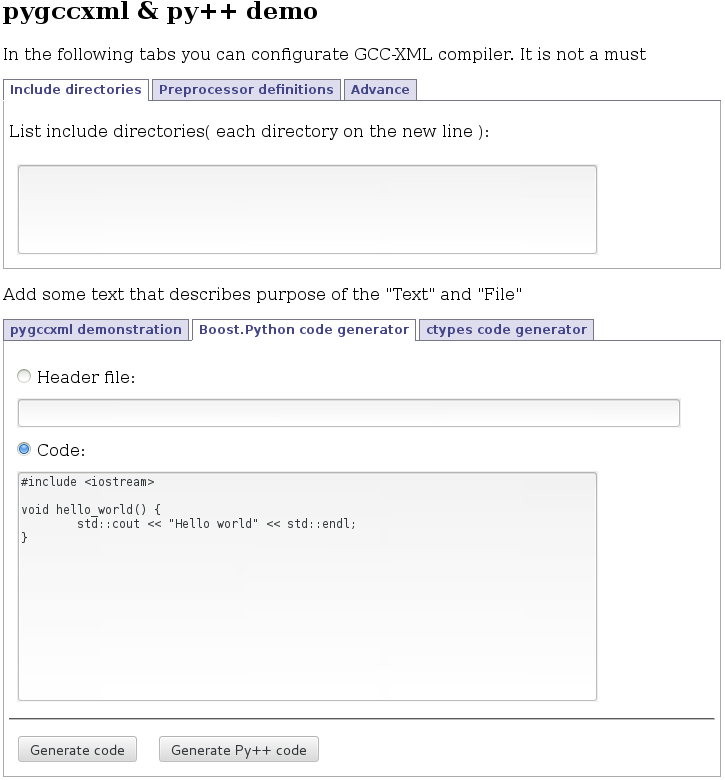
\includegraphics[width=0.72\textwidth]{exemples/pyplusplus/ihm.png}
    \caption{Interface web de Py++}
    \label{fig:pyplusplusihm}
\end{figure*}

\subsection{Analyse}

\subsubsection{Intérêts de l'utilisation de Py++}

Il n'y a aucun code supplémentaire à écrire, il suffit de lancer l'outil. Cela permet de ne pas avoir de code à maintenir, car il suffira de relancer le générateur à chaque modification de structure du code.

\subsubsection{Limites de l'utilisation de Py++}

Il faut relancer Py++ à chaque modification pour actualiser le code modifié. Il ne détecte pas les modèles qui n'ont pas été instanciées. Ceci est due au fait que Py++ utilise GCCXML pour extraire la structure du code. Or il s'avère que le projet GCCXML n'a pas besoin de modèles non instanciées \footnote{\url{https://gccxml.github.io/HTML/FAQ.html}}.

\section{Utilisation des CTypes}

Cette partie a été écrite en utilisant la documentation officielle des CTypes\cite{pythonctypes}.

\subsection{Présentation}

Ctypes est une bibliothèque de fonction étrangères pour Python. Cela permet d'avoir des types de données compatible avec le langage C et également d'appeler des fonctions présentes dans les DLLs ou bibliothèques partagées. Cette bibliothèque peut être utilisée comme interface entre ces bibliothèques et du code Python. Il est donc possible de charger directement une bibliothèque existante avec ce système.

L'article \cite{2008ACLWCFTTGuy} donne un exemple de génération automatique de code utilisant les CTypes avec les bibliothèques h2xml et xml2py. Malheureusement, nous n'avons pas pu reproduire ces résultats.

On allons donc vous présenter un exemple qui a été écrit manuellement :

\lstinputlisting[style=customc,caption={Exemple C++ utilisé},label=ctypesexemple]{exemples/ctypes/myexample.cpp}

\lstinputlisting[style=custombash,caption={Commandes utilisées pour exécuter l'exemple},label=ctypescommande]{exemples/ctypes/commande}

\lstinputlisting[style=custompython,caption={Test Python des Ctypes},label=ctypestest]{exemples/ctypes/test.py}

À la ligne 3 de \ref{ctypesexemple}, on remarque qu'il y a l'ajout de \emph{extern "C"}. Cet ajout est obligatoire pour de la compilateur n'ajoute pas de décorations sur les méthodes. Pour utiliser les CTypes, il faut tout d'abord compiler le code C++ sous la forme d'une extension. Puis, on peut utiliser l'extension comme \ref{ctypestest}. La variable \emph{testlib} contient toutes les méthodes de l'extension et elles sont utilisables comme un objet.

\subsection{Analyse}

\subsubsection{Intérêts de l'utilisation des CTypes}

Il s'agit de la solution la plus rapide et la plus simple en terme de création et d'éxécution du code. En effet, il n'est pas nécessaire d'écrire une interface entre le code C++ et Python. À l'aide des CTypes, on peut exécuter directement les fonctions présentes dans une bibliothèque partagée.

\subsubsection{Limites de l'utilisation des CTypes}

Les CTypes ne supportent pas l'instanciation de modèles. De plus pour rendre utilisable les fonctions, il est nécessaire d'ajouter \emph{extern "C"} sur le prototype des fonctions. Il n'est aussi pas possible d'avoir un support des namespaces ou des classes. En effet, toutes les fonctions doivent être accessible directement à partir de la bibliothèque. Les CTypes auraient pu être intéressant si DGtal avait été écrite en C car les CTypes ont été initialement pensés pour être utilisés en C.

\section{Utilisation de l'arbre de syntaxe C++}

Cette partie a été rédigée à l'aide de l'article \cite{2014IACGWLTamas}.

\subsection{Présentation}

L'arbre de syntaxe aussi appelé AST \emph{Abstract Syntax Tree} permet d'obtenir la structure du code C++. Nous avons extrait cette structure avec le compilateur Clang, nous avons choisi ce compilateur car il représente également les modèles non instanciés. De plus Clang est un compilateur C/C++ qui ce veut plus personnalisable que les équivalents tel que GCC \cite{clangmain}. Grâce à cet arbre, nous pouvons générer automatiquement les interfaces nécessaires à l'utilisation de SWIG ou Boost.Python.

\lstinputlisting[style=customPython,caption={Code Python nécessaire à la génération de l'AST},label=clangdumpast]{propositions/clang/dump_ast.py}

\lstinputlisting[style=customc,caption={Code d'exemple c++ avec une modèle},label=clangexemple]{propositions/clang/myexample.h}

\lstinputlisting[style=custombash,caption={AST généré},label=clangastresultat]{propositions/clang/arbreACT.txt}

Grâce au script \ref{clangdumpast}, on peut générer l'arbre de syntaxe \ref{clangastresultat} de l'exemple \ref{clangexemple}.

\subsubsection{Intérêts de l'utilisation de l'arbre de syntaxe C++}

La combinaison de l'arbre syntaxique et du compilateur Clang, nous permettrais de créer un outil. Cet outil pourrait générer automatiquement le code d'interface nécessaire à l'utilisation de SWIG ou Boost.Python.

\subsubsection{Limites de l'utilisation de l'arbre de syntaxe C++}

L'utilisation de l'arbre de syntaxe C++ ne règle pas le problème des modèles. En effet, il faut toujours les instancier pour pouvoir les utiliser.

\section{Récapitulatif}

Nous avons préparé un tableau récapitulatif \ref{tab:Comparatif} qui contient les différents critères permettant de différencier les solutions d'interfaçage de C++ en Python. Nous avons fusionné Py++ et Boost.Python car il s'agit de la même solution à savoir Boost.Python. Nous n'avons pas inclus la solution qui parlait de l'utilisation de l'arbre syntaxique C++ car elle n'est pas comparable avec les autres.

\begin{table*} % Utiliser la version étoilée des flottants pour les faire tenir sur deux colonnes
    \begin{center}
        \begin{tabular}{|p{5cm}||c|c|c|}
            \hline
                                                            & SWIG      & Boost.Python  & CTypes    \\
            \hline
            \hline
Peut convertir en d'autres langages que Python              & $\surd$   &               &           \\
            \hline
Possède des générateurs d'interface                         & $\surd$   & $\surd$       &           \\
            \hline
Documentation complète sur tous les éléments du langage C++ & $\surd$   &               &           \\
            \hline
Exhaustivité de la documentation                            & Bonne      & Légère pour les fonctions avancées          & Légère         \\
            \hline
Support du C++                                              & Quasi complet & Total     & Aucun (support du C)    \\
            \hline
Support des modèles                                       & Via instanciation & Via instanciation & Non \\
            \hline
        \end{tabular}
    \end{center}
    \caption{Tableau comparatif des avantages des interfaceurs de C++ en Python}
    \label{tab:Comparatif}
\end{table*}

\section{Conclusion}

À l'issue de ce travail de recherche bibliographique, il apparaît que plusieurs propositions peuvent servir de base à la résolution de notre problème.

Il semble se détacher un certain nombre de directions privilégiées que nous allons exploiter en priorité dans nos propositions. Celles-ci font l'objet de l'étude du chapitre suivant.

%-------------------------------------------------------------------------------------------------------------

% \part{Réalisations} % À décommenter si l'état de l'art a nécessité plusieurs chapitres.
% \label{part:Realisations}

\chapter{Proposition}
\label{chap:Proposition}

A l'aide de notre état de l'art, nous avons pu formuler la proposition suivante :

\section{Utiliser l'arbre syntaxique (AST) donné par le compilateur Clang pour générer les interfaces nécessaires à SWIG}

%\subsection{Idées préliminaires}

Lors de notre état de l'art, nous avons identifié trois méthodes utilisables pour générer des modules Python : SWIG, Boost.Python et CTypes. Nous écartons d'emblée CTypes car son utilisation est orientée vers le langage C, et, bien qu'il soit possible de développer une sur-couche afin de prendre en compte les éléments du C++, cela serait trop coûteux en temps et peu intéressant par rapport à ce qu'offre les autres solutions.

SWIG et Boost.Python nécessitent l'écriture d'une interface pour faire le lien entre le code Python et le code C++. La principale différence entre SWIG et Boost.Python est que SWIG est plus à jour et permet de générer du code autre que Python une fois l'interface écrite. La documentation est également plus à jour et plus précise. Ce sont ces éléments qui ont motivé notre décision d'opter pour SWIG.

Étant donné que la solution proposée ne doit pas ajouter de code supplémentaire à gérer, nous allons mettre en place une solution d'automatisation de génération d'interface. Nous avons comparé différentes méthodes pour extraire la structure du code. Nous avons trouvé deux méthodes utilisables à savoir GCCXML et Clang. Nous avons sélectionné Clang car il extrait également la structure des modèles non instanciés.

Il reste à régler le problème des modèles. En effet, il faut connaître le type attribué à leurs arguments avant de les instancier, nous proposons d'intégrer les types les plus susceptibles d'êtres utilisés dans la documentation Doxygen de la classe. Ainsi, nous pourrons récupérer ces types afin de générer les classes correspondant aux modèles.

%\subsection{Formalisation}

%\subsection{Démonstration}

%\subsection{Analyse}

%\section{\emph{<Notre proposition \textit{i}>}}

%L'organisation des cette section (voire chapitre) est la plus libre qui soit. Toutefois, on peut proposer une organisation qui distingue l'intuition de sa formalisation et de sa démonstration.

%\subsection{Idées préliminaires}

%La fin du chapitre~\ref{chap:EtatArt} a permis de mettre en avant les éléments présents dans des propositions antérieures qui sont exploitables pour résoudre notre problème. Nous développons ici les idées qui nous semblent les plus à même d'y parvenir.

%\subsection{Formalisation}

%Le développements des intuitions et idées de la section précédente vont aboutir à des propositions formalisées. Cela peut se traduire aussi bien par des formules que des algorithmes.

%\emph{Nous avons trouvé une formule particulièrement pertinente pour résumer les nombreuses caractéristiques d'une image :}
%\begin{equation}
%	\label{eq:Proposition}
%	\Phi :
%		\begin{array}{ccc}
%			T_1 \times \ldots \times T_n & \to & \mathbb{R}\\
%			(a, p, m_1, m_2, \kappa, \ldots, \alpha, \alpha', \ldots,z) & \mapsto & \ldots
%		\end{array}
%\end{equation}

%\emph{Les différents paramètres de la fonction sont eux-mêmes fournis par l'algorithme~\ref{alg:Proposition}.}

%\begin{algorithm*}
%	L'algorithme peut être décrit de différentes manières, avec les environnements :
%	\begin{itemize}
%		\item verbatim :
%			\begin{verbatim}
%fonction F (I : image) : (T1, T2, ..., Tn)
%...
%			\end{verbatim}
%		\item tabbing :
%			\begin{tabbing}
%				\textbf{fonction} $F$ ($I : \mathcal{I}$) : $T_1 \times T_2 \times \cdots \times T_n$\\
%				...
%			\end{tabbing}
%		\item algorithmic :
%			\begin{algorithmic}[1]
%				\REQUIRE $n \geq 0$
%				\ENSURE $y = x^n$
%				\STATE $y \Leftarrow 1$
%				\STATE $X \Leftarrow x$
%				\STATE $N \Leftarrow n$
%				\WHILE{$N \neq 0$}
%					\IF{$N$ is even}
%						\STATE $X \Leftarrow X \times X$
%						\STATE $N \Leftarrow N / 2$
%					\ELSE[$N$ is odd]
%						\STATE $y \Leftarrow y \times X$
%						\STATE $N \Leftarrow N - 1$
%					\ENDIF
%				\ENDWHILE
%			\end{algorithmic}
%		\item voire avec les environnement standards et/ou en français.
%	\end{itemize}
%	\caption{Proposition}
%	\label{alg:Proposition}
%\end{algorithm*}

%\subsection{Démonstration}

%Tous les éléments de démonstration du bien fondé de la méthode proposée doivent être explicités si ce n'est sous la forme de théorèmes, du moins avec un enchaînement argumenté de causes à effets.

%\begin{theoreme}
%	Soit $(a, p, m_1, m_2, \kappa, \ldots, \alpha, \alpha', \ldots,z) \in T_1 \times \ldots \times T_n$ tel que ... alors ...
%\end{theoreme}

%\begin{preuve}
%	Procédons par contradiction. ...~\hfill$\square$
%\end{preuve}

%\subsection{Analyse}

%Une analyse objective sur cette orientation est ici faite. Le problème est-il résolu dans sa totalité, sinon quelle partie ? La résolution est-elle efficace d'un point de vue informatique ? Etc.

%\section{Conclusion}

%Différentes idées nous ont conduit à faire différentes propositions. À ce stade, il convient de restreindre leur nombre afin d'avoir le temps de conduire des expérimentations suffisamment poussées, nous permettant d'établir des conclusions pertinentes.

%\emph{En comparant les apports démontrés ou à vérifier dans le tableau ..., nous en déduisons un classement << au mérite >> qui est le suivant : .... Par manque de temps, nous allons nous limiter aux deux premiers dans le chapitre~\ref{chap:Experimentations}.}

%-------------------------------------------------------------------------------------------------------------

%\chapter{Expérimentations et résultats}
%\label{chap:Experimentations}


%\section{Conclusion}

%-------------------------------------------------------------------------------------------------------------

\chapter{Conclusion}

Tout d'abord, nous vous rappelons que notre objectif est d'intégrer un interpréteur Python au sien de la librairie DGtal.

Nous avons exploré dans ce document les différentes solutions pour utiliser une bibliothèque développée en C++ avec le langage Python. 
SWIG et Boost.Python permettent de mettre en place ce genre de solution mais impliquent un développement supplémentaire et ne gèrent pas les modèles de façon optimale.

Nous avons proposé une solution en combinant la puissance de SWIG et du compilateur Clang.

Nous possédons maintenant les connaissances nécessaires au passage de la prochaine étape : le développement.

\section{Enseignements}
Nous avons tiré des enseignements au niveau du déroulement d'un projet de recherche et développement, pour la partie d'étude bibliographique.

Nous connaissions déjà les technologies utilisés, mais pas sous cet angle. Ce projet nous a donc fait monter en compétence sur les interactions entre les technologies de programmation en général et de façon plus précise sur C++ et Python.

%---------------------------------------------------------------------------------------------------------

\printbibliography{}

\listoffigures{}

\listoftables{}

%\listofalgorithms{}

\appendix

%\chapter{Rappels}
%\label{ann:Rappels}

%\chapter{Mesures détaillées}
%\label{ann:Mesures}


\chapter{Fiches de lecture}
\label{ann:FichesLecture}

\section{\emph{Python scripting for computational science}}

Ce livre \cite{2007PSFCSHans} explique les avantages de l'utilisation de Python pour faire du calcul scientifique. Nous nous sommes intéressé à la partie qui explique comment faire appel à des fonctions c++ dans Python.

\subsection{Résumé}

L'auteur nous apprend les techniques déjà existantes pour interfacer du C++ avec Python. Il aborde les techniques suivantes :
\begin{enumerate}
\item F2PY, Weave, Instant (avec un exemple)
\item SWIG (avec des exemples)
\item Boost.Python, SCXX, CXX (seulement évoquées)
\end{enumerate}

\subsection{Analyse}

Nous sommes toujours au commencement de nos recherches, nous allons donc étudier en détail les différentes techniques abordées par l'auteur.

\section{\emph{Reflection-based Python-c++ bindings}}

Cet article \cite{2004RBPCBGenrowicz} traite des deux principales méthodes pour interfacer du c++ avec du Python.

\subsection{Résumé}

Les principaux problèmes pour interfacer du c++ avec du Python sont les suivants :
\begin{enumerate}
\item \emph{Objets et conversion de paramètres} : les arguments et les valeurs de retour des fonctions doivent être passé d'un langage à l'autre.
\item \emph{Types manquants ou incomplet} : la signature des fonctions et des classes peut inclure des types qui sont seulement déclarés et pas définis.
\item \emph{Gestion de la mémoire} : Python possède un ramasse miette alors que C++ demande une gestion de la mémoire à la main.
\item \emph{Redéfinition de fonctions c++} : Python n'a pas besoin de ce système étant donné qu'il est typé dynamiquement.
\item \emph{Modèles C++} : Une convention de nommage est requise pour distinguer les modèles.
\end{enumerate}

Il existe deux manière d'interfacer du C++ avec du Python :
\begin{enumerate}
\item \emph{Static Wrapping} : Cette technique consiste à écrire du code entre le code Python et c++ pour déclarer la liste des méthodes utilisées avec leurs paramètres. L'inconvénient de cette méthode est qu'il est très long et fastidieux d'écrire ce code. Il existe déjà des bibliothèques qui implémentent cette technique. SWIG et Boost.Python sont les plus populaires.
\item \emph{Dynamic Wrapping} : Cette technique consiste à s'appuyer sur un dictionnaire de type pour exécuter directement sur C++ dynamiquement à l'exécution. L'avantage est qu'il n'y a pas à écrire de code supplémentaire. Cette technique est implémenté par PyLCGDict et PyROOT.
\end{enumerate}

\subsection{Analyse}

Cet article nous a permis d'avancer dans notre réflexion. Nous allons essayer de voir ce que donne les deux techniques (statique et dynamique en pratique).

\section{\emph{A Python Extension to the ATLAS Online Software for the Thin Gap Chamber Trigger System}}

Il s'agit d'un article scientifique \cite{2004APETTAOSFTTGCTSTadashi} qui utilise montre un exemple pratique de l'utilisation de Python comme passerelle entre applications.

\subsection{Résumé}

Dans cet article, les auteurs ont fait le choix de Boost.Python pour interfacer une application c++ avec Zope un cadriciel web Python. Cela leurs a permis d'avoir accès à ATLAS Online dans leur site internet.

\subsection{Analyse}

On pourrait penser que cet article n'a pas beaucoup d'intérêts. Mais, il faut voir que l'article date de 2004. Il faudra donc vérifier si l'on a encore des innovations à faire dans ce domaine.

\section{\emph{Using SWIG to bind C++ to Python}}

Cet article \cite{2003USTBCTPTeresa} est un manuel qui explique le fonctionnement de SWIG.

\subsection{Résumé}

Cet article explique en détail les différentes parties du langage C++ qu'il est possible de passer en Python avec SWIG. SWIG est une passerelle de type statique. Pour utiliser SWIG, il faut écrire un fichier d'interface qui fait l'intermédiaire entre le code C++ et l'interpréteur Python.

Voici la liste des fonctions qu'il est possible de passer de C++ à l'interpréteur Python :
\begin{enumerate}
\item \emph{Les fonctions simple}.
\item \emph{La redéfinition de fonctions}.
\item \emph{Les classes C++}.
\item \emph{Les arguments par défaut}.
\item \emph{L'ordre des arguments} : Python est plus flexible que C++, il est possible de choisir l'argument que l'on veut utiliser. En effet, s'il existe une méthode \emph{action(int a=5,int b=8)}, il est possible de l'utiliser en avec uniquement l'argument b tel que \emph{action(b=9)}.
\item \emph{La redéfinition d'opérateur}.
\item \emph{Les modèles C++}.
\item \emph{Les exceptions}.
\end{enumerate}

Il est également possible de d'étendre SWIG. Il est possible de créer des macros pour écrire des fichiers d'interface plus court.

\subsection{Analyse}

Cet article explique bien le fonctionnement de SWIG. Malheusement, il n'est pas très à jour, il vaut mieux utiliser la documentation de SWIG qui est plus complète.

\section{\emph{Creating a Python GUI for a C++ Image Processing Library}}

Cet article \cite{2004CAPGFACIPLWuth} est un retour d'expérience sur l'élaboration d'une interface graphique en Python pour une bibliothèque en C++.

\subsection{Résumé}

L'objectif du travail des chercheurs aillant rédigé l'article était de créer une interface graphique utilisant Python et Tkinter pour la bibliothèque de manipulation d'images IPL98, écrite en C/C++.
L'utilisation de Python pour créer l'interface graphique est due à sa simplicité et sa rapidité d'utilisation par rapport aux bibliothèques graphiques C++.
Afin de gérer l'interfaçage entre la bibliothèque C++ et Python, l'équipe a utilisé SWIG, qui permet d'utiliser des fonctions C++ en rédigeant des interfaces spécifiques. Il leur est vite apparu qu'interfacer l'intégralité de la librairie IPL98 était très complexe sinon impossible, et ce pour plusieurs raisons :

\begin{enumerate}
\item L'interface SWIG, devant être générée manuellement, serait bien trop complexe à maintenir.
\item La disimilarité entre les langages (types de structure, modèles d'objets, etc.) rendrait la bibliothèque Python différente de celle d'origine, ce qui impliquerait de rédiger de la documentation supplémentaire pour la version Python.
\item La gestion de mémoire devient bien plus compliquée lorsque des objets et des pointeurs sont manipulés entre les deux langages.
\end{enumerate}

La solution apportée est d'écrire des fonctions C++ réalisant des tâches spécifiques, et qui seront elles interfacées avec Python. Ainsi, si la totalité de la bibliothèque n'est pas utilisable, via Python, on peut porter des fonctionnalité individuellement par des fonctions C++.
Parmi les avantages de cette solution, on peut citer la simplicité de mise en oeuvre, la disparition des problèmes de mémoire, et l'indépendance des différents modules.
Cependant, cette solutions présente également des défauts : pas d'accès direct aux objets créé car si ils sont détruits après l'exécution de la fonction C++ appelée par Python, et donc, une plus grande complexité pour les fonctionnalités nécessitant une interaction utilisateur (sélectionner un pixel par exemple)

\subsection{Analyse}

Les besoins exprimés par l'équipe de recherche dans cet article sont similaire à ce de ce projet, car ils nécessitent une interface entre Python et C++.

\section{Automatic C Library Wrapping - Ctypes from the trenches}

cet article \cite{2008ACLWCFTTGuy} utilise un exemple de d'utilisation de wrapping Python avec le framework little CMS. 

\subsection{Résumé}

L'auteur souligne l'importance des Ctypes pour effectuer la transformation de c++ à Python. Boost.Python est intéressant à utiliser si l'on veut utiliser une API plus complète en C++ qui reflète également la nature objet du code comme l'héritage. Cython est utile si l'on souhaite améliorer les performances de Python sur certaine partie du code. SWIG est intéressant si l'on souhaite utiliser le code original dans différents langages.

Il existe différents outils pour générer le code nécessaire à utilisation des englobeurs tel que Py++ pour Boost.Python et h2xml.py et xml2py.py pour les CTypes. L'auteur à choisit d'utiliser les CTypes pour 3 raisons :
\begin{enumerate}
\item L'ubiquité comme approche de liaison, étant donné que ctype fait partie de la distribution par défaut.
\item Il n'y a pas de compilation du code natif en bibliothèque de nécessaire. De plus ce système se base sur l'installation outil de développement et la bibliothèque d'englobement et vu comme une plateforme indépendante.
\item L'utilisation d'un générateur de code pour automatiser des grandes parties de l'englobement du code rend le système robuste contre les modifications.
\end{enumerate}

À la fin de l'article, l'auteur explique qu'il lui a fallu 15 minutes pour mettre à jour son code lorsque qu'une nouvelle version de \emph{little CMS} est sortie.

\subsection{Analyse}

Cette approche d'utiliser h2xml.py et xml2py.py semble intéressante car elle répond à notre besoin. Nous allons ajouter cette méthode à notre comparatif pour voir la différence avec les autres.

\section{Implementing a code generator with libclang}

Cet article \cite{2014IACGWLTamas} montre qu'il est possible d'utiliser le compilateur clang pour générer le code intermédiaire pour Boost.Python.

\subsection{Résumé}

L'avantage d'utiliser clang pour générer le code intermédiaire est qu'il est facile de mettre à jour l'interface SWIG ou Boost.Python. Dans l'article, l'auteur se concentre sur une classe simple, à laquelle il va générer le code de l'interface avec LLVM. Cette technique est utilisé car le langage C++ manque de système d'introspection évolué. Normalement, pour cette génération, il faut que le projet suive des règles strictes lors de lors du codage mais libclang permet de s'affranchir de cette contrainte. 

L'auteur explique ensuite que pour générer l'interface, il extrait l'arbre AST (abstract syntax tree). Cela permet d'avoir toutes les informations sur le code et d'appliquer une transformation aux noeuds. Sur chaque noeuds, qui va représenter une méthode, une classe, une fonction va être appliqué pour générer l'interface.

\subsection{Analyse}

Cette approche est intéressante et elle nous offre une alternative à Py++. On pourrait également utiliser cette méthode pour générer du code SWIG ce qui permettrait de rendre le code utilisable sur d'autres plateformes que Python.

\chapter{Planification}

La figure~\ref{fig:PlanningPrevisionnel} présente le planning prévisionnel élaboré au début du projet. Nous avons choisi une période de 4 semaines pour l'étude bibliographique car bien que nous ayons des connaissances en C++ et Python, une documentation était nécessaire afin de monter en compétence sur les différentes manières d'interfacer les deux langages. De plus, il faut ajouter la prise de connaissances sur la bibliothèque DGtal. Ensuite, nous avons mis 3 semaines pour l'analyse des solutions car nous anticipions d'en trouver un nombre important, la comparaison nous aurait donc pris du temps. Le planning effectif ~\ref{fig:PlanningEffectif} montre que nous avons du étendre notre phase de recherche bibliographique. En effet bien que nous n'ayons pas eu de problèmes pour trouver des solutions exploitables, celles-ci se sont avérées anciennes et/ou peu documentées. Cela nous a forcé à fournir un comparatif de solutions moins étendues mais plus récentes.

\begin{figure*}
% - Utiliser la version étoilée des flottants pour les faire tenir sur deux colonnes
% - éventuellement utiliser la conditionnelle \ifscreen ... \else ... \fi pour orienter
%   correctement le planning en fonction de l'orientation du papier (cf. ci-dessous)
%   pour l'autoévaluation.
	\centering
	
        \begin{ganttchart}[
            link/.style={-latex, line width=1.8pt},
            vgrid={draw=none, dotted},
            y unit chart=.75cm,
            y unit title=.6cm,
            x unit=0.6cm,
            bar height=.5,
            newline shortcut=true,
            bar label node/.append style={align=right},
            %group height=.2,
            %milestone height=.5,
            milestone label node/.append style={xshift=-6pt},
            bar label node/.append style={xshift=-6pt},
            group label node/.append style={xshift=-6pt},
          ]{1}{19}
          %\setganttlinklabel{f-s}{}
          \gantttitle{PRED}{19}\\
          \gantttitle[]{2014}{12}
          \gantttitle[]{2015}{7}\\
          
          \gantttitlelist{41,...,52}{1}
          \gantttitlelist{1,...,7}{1}\\
        
          \ganttgroup{Acquisition du sujet}{1}{1}\\
        
          
          %\ganttmilestone{kick off meeting}{0}\\
          %\ganttmilestone{project meetings}{4}
          %\ganttmilestone{}{8}
          %\ganttmilestone{}{12}
          %\ganttmilestone{}{16}
          %\ganttmilestone{}{20}\\
          %\ganttmilestone{final review}{24}\\
        
          \ganttgroup{Étude bibliographique}{2}{5}\\
         
        
          \ganttbar[name=recherche]{Recherche d'articles\\{\scriptsize Recherche et lectures d'articles scientifiques}}{2}{5}\\
          \ganttbar[name=dgtal]{Prise en main de DGTal\\{\scriptsize Installation, compilation et compréhension de DGTal}}{2}{5}\\
          \ganttbar[name=esai]{Essai de solutions\\{\scriptsize Tests de solutions existantes}}{2}{5}\\
        \ganttbar[name=vacs]{Vacances}{4}{4}\\
          \ganttgroup{Analyse des solutions}{6}{8}\\
        
          \ganttbar[name=T2.1]{Comparatif\\{}}{6}{8}\\
          \ganttbar[name=T2.2]{Validation\\{}}{6}{8}\\
          \ganttmilestone{Soutenance}{8}\\
          %\ganttlink{T2.1}{T2.2}
          %\ganttlink[link mid=.159]{T2.1}{T2.3}
          %\ganttlink[link type=f-s]{T2.3}{T2.4}
        %  \ganttlink{elem15}{elem17}
        
          %\ganttgroup{WP3. Experiments}{7}{9}
          \ganttgroup{Développement}{10}{19}\\
        
          \ganttbar[name=T3.1]{Développement\\{}}{10}{11}
          \ganttbar[name=dev3]{}{14}{15}\\
          \ganttbar[name=T3.1]{Vacances\\{}}{12}{13}\\
          \ganttbar[name=T3.1]{Validations et finalisations\\{}}{16}{18}\\
          \ganttmilestone{Soutenance}{19}\\
          %\ganttbar[name=T3.3]{task 3.3\\{\scriptsize large-scale experimentation}}{19}{24}
        \end{ganttchart}
	\caption{Planification prévisionnelle}
	\label{fig:PlanningPrevisionnel}
\end{figure*}


\begin{figure*}
	\centering
		  \begin{ganttchart}[
            link/.style={-latex, line width=1.8pt},
            vgrid={draw=none, dotted},
            y unit chart=.75cm,
            y unit title=.6cm,
            x unit=0.6cm,
            bar height=.5,
            newline shortcut=true,
            bar label node/.append style={align=right},
            milestone label node/.append style={xshift=-6pt},
            bar label node/.append style={xshift=-6pt},
            group label node/.append style={xshift=-6pt},
          ]{1}{19}
          \gantttitle{PRED}{19}\\
          \gantttitle[]{2014}{12}
          \gantttitle[]{2015}{7}\\
          
          \gantttitlelist{41,...,52}{1}
          \gantttitlelist{1,...,7}{1}\\
        
          \ganttgroup{Acquisition du sujet}{1}{2}\\
          \ganttbar{\\Mise en place du projet}{1}{2}\\
        
        %groupe biblio
          \ganttgroup{Étude bibliographique}{2}{8}\\
        
          \ganttbar[name=recherche]{Recherche d'articles\\{\scriptsize Recherche et lectures d'articles scientifiques}}{2}{6}\\
          \ganttbar[name=dgtal]{Prise en main de DGTal\\{\scriptsize Installation, compilation et compréhension de DGTal}}{2}{8}\\
          \ganttbar[name=esai]{Essai de solutions\\{\scriptsize Tests de solutions existantes}}{4}{8}\\
        \ganttbar[name=vacs]{Vacances}{4}{4}\\
        
        %groupe analyse des solutions
          \ganttgroup{Analyse des solutions}{7}{8}\\
        
          \ganttbar[name=T2.1]{Comparatif\\{}}{7}{8}\\
          \ganttbar[name=T2.2]{Validation\\{}}{7}{8}\\
          \ganttmilestone{Soutenance}{8}\\
        
        \end{ganttchart}
	\caption{Planning effectif}
	\label{fig:PlanningEffectif}
\end{figure*}

\chapter{Fiches de suivi}
\label{ann:FichesSuivi}

\begin{fichesuivi}{6 octobre 2014}{12 octobre 2014}
	\tempstravailA{3}{00}
	\tempstravailB{3}{00}

	\begin{travaileffectue}
		\begin{itemize}
            \item Recherche bibliographique réalisée à 5\% ;
            \item Compilation de DGtal fonctionne mais impossible d'utiliser la librairie ITK ;
            \item Test de certains exemple de DGtal ;
            \item Configuration de l'environnement de travail c9.io ;
            \item Rappel sur la syntaxe de Python ;
            \item Mise en place d'un git pour le stockage des rapports https://github.com/CoreFloDev/Pred2014-DGtal.
		\end{itemize}
	\end{travaileffectue}

	\begin{travailnoneffectue}
		\begin{itemize}
			\item Rendre le rapport hebdomadaire.
		\end{itemize}
	\end{travailnoneffectue}

	\begin{echange}
		\begin{itemize}
			\item Réunion de présentation avec Nicolas Normand.
		\end{itemize}
	\end{echange}

	\begin{planification}
		\begin{itemize}
			\item Travail à avancer sur la bibliographie ;
            \item Mise en place du rapport final sur github en latex.
		\end{itemize}
	\end{planification}
\end{fichesuivi}

\begin{fichesuivi}{13 octobre 2014}{19 octobre 2014}
	\tempstravailA{8}{00}
	\tempstravailB{5}{00}

	\begin{travaileffectue}
    	\begin{itemize}
            \item Recherche bibliographique et écriture d'une fiche de lecture ;
            \item Mise en place du rapport de Pred en latex ;
            \item Test de différentes techniques de communication entre c++ et Python par l'utilisation de librairies.
            \item Début de l'analyse de DGtal ;
            \item Test des exemples de DGtal ;
            \item Mise en place d'un nouveau système de communication entre binome.
        \end{itemize}
	\end{travaileffectue}

	\begin{travailnoneffectue}
	\end{travailnoneffectue}

	\begin{echange}
	    \begin{itemize}
	        \item Bref échange de 5 min sur l'avancement.
	    \end{itemize}
	\end{echange}

	\begin{planification}
	    \begin{itemize}
	        \item Analyse de DGtal ;
            \item État de l'art des techniques de communication avec Python.
        \end{itemize}
	\end{planification}
\end{fichesuivi}

\begin{fichesuivi}{20 octobre 2014}{26 octobre 2014}
	\tempstravailA{7}{00}
	\tempstravailB{6}{00}

	\begin{travaileffectue}
	    \begin{itemize}
	        \item Recherche et lecture de nouveaux articles scientifiques ;
            \item Étude d'un exemple de DGtal.
        \end{itemize}
	\end{travaileffectue}

	\begin{travailnoneffectue}
	\end{travailnoneffectue}

	\begin{echange}
	    \begin{itemize}
	        \item Réunion d'une heure.
	    \end{itemize}
	\end{echange}

	\begin{planification}
    	\begin{itemize}
    	    \item Fiches de lectures pour les articles scientifiques trouvés ;
            \item Comparatif des différentes méthodes d'interfaçage entre C++ et Python ;
            \item Planning prévisionnel.
        \end{itemize}
	\end{planification}
\end{fichesuivi}

\begin{fichesuivi}{27 octobre 2014}{2 novembre 2014}
	\tempstravailA{8}{00}
	\tempstravailB{6}{00}

	\begin{travaileffectue}
	    \begin{itemize}
	        \item réalisation des fiches de lecture des articles trouvés.
	    \end{itemize}
	\end{travaileffectue}

	\begin{travailnoneffectue}
	\end{travailnoneffectue}

	\begin{echange}
	\end{echange}

	\begin{planification}
	\end{planification}
\end{fichesuivi}

\begin{fichesuivi}{3 novembre 2014}{9 novembre 2014}
	\tempstravailA{10}{00}
	\tempstravailB{8}{00}

	\begin{travaileffectue}
	    \begin{itemize}
	        \item comparatif des méthodes de création d'extension Python à partir de code C++;
            \item ajout de biblatex dans le document latex;
            \item ajout de la coloration du code dans le rapport Latex;
            \item réalisation du planning prévisionnel avec un gantt latex.
	    \end{itemize}
	\end{travaileffectue}

	\begin{travailnoneffectue}
	\end{travailnoneffectue}

	\begin{echange}
	\end{echange}

	\begin{planification}
	\end{planification}
\end{fichesuivi}

\begin{fichesuivi}{10 novembre 2014}{16 novembre 2014}
	\tempstravailA{6}{30}
	\tempstravailB{8}{00}

	\begin{travaileffectue}
	    \begin{itemize}
	        \item écriture d'une nouvelle fiche de lecture ;
            \item comparatif des méthodes d'interfaçage entre C++ et Python complété à 70\% ;
            \item difficultés à faire fonctionner h2xml et xml2py ;
            \item analyse de la structure de DGtal ;
            \item commencement de l'intégration d'une classe de DGtal avec boost.Python ;
            \item structure globale (introduction, conclusion, transitions) du rapport à  25\%.
	    \end{itemize}
	\end{travaileffectue}

	\begin{travailnoneffectue}
	\end{travailnoneffectue}

	\begin{echange}
    	\begin{itemize}
    	    \item réunion de 1 heure le 14/11.
    	\end{itemize}
	\end{echange}

	\begin{planification}
	    \begin{itemize}
    	    \item  analyser le fonctionnement de CLANG pour générer du code d'interface utilisable par boost.Python ou SWIG;
            \item faire une version présentable du rapport.
	    \end{itemize}
	\end{planification}
\end{fichesuivi}

\begin{fichesuivi}{17 novembre 2014}{23 novembre 2014}
	\tempstravailA{10}{00}
	\tempstravailB{10}{00}

	\begin{travaileffectue}
	    \begin{itemize}
	        \item Intégration d'un modèle à l'exemple de Boost.Python et SWIG ;
            \item tableau comparatif des méthodes d'interpolation avec Python ;
            \item lecture d'articles sur les modèles C++ et leur fonctionnement détaillé;
            \item rédaction de la présentation de DGtal.
	    \end{itemize}
	\end{travaileffectue}

	\begin{travailnoneffectue}
	\end{travailnoneffectue}

	\begin{echange}
	\end{echange}

	\begin{planification}
	    \begin{itemize}
	        \item recherches plus approfondies sur CLANG, les Ctype, l'API C Python et les RTTI ;
            \item fournir une version aboutie du rapport ;
            \item rédaction de bibliographie sur le fonctionnement interne de SWIG et Boost.Python.
	    \end{itemize}
	\end{planification}
\end{fichesuivi}

\begin{fichesuivi}{24 novembre 2014}{30 novembre 2014}
	\tempstravailA{13}{00}
	\tempstravailB{13}{00}

	\begin{travaileffectue}
	    \begin{itemize}
	        \item Rapport final ;
            \item Planning actualisé ;
            \item Ajout d'une partie sur les CTypes ;
            \item Ajout d'une partie sur CLang
            \item Ajout fiche auto évaluation ;
            \item Correction des fautes du rapport.
	    \end{itemize}
	\end{travaileffectue}

	\begin{travailnoneffectue}
	\end{travailnoneffectue}

	\begin{echange}
	    \begin{itemize}
	        \item Envoie d'une version préliminaire du rapport le 28/11.
	    \end{itemize}
	\end{echange}

	\begin{planification}
	    \begin{itemize}
	        \item Diaporama de présentation.
	    \end{itemize}
	\end{planification}
\end{fichesuivi}

\begin{fichesuivi}{}{}
	\tempstravailA{21}{40}
	\tempstravailB{17}{10}

	\begin{travaileffectue}
	\end{travaileffectue}

	\begin{travailnoneffectue}
	\end{travailnoneffectue}

	\begin{echange}
	\end{echange}

	\begin{planification}
	\end{planification}
\end{fichesuivi}

\begin{fichesuivi}{}{}
	\tempstravailA{4}{30}
	\tempstravailB{8}{15}

	\begin{travaileffectue}
	\end{travaileffectue}

	\begin{travailnoneffectue}
	\end{travailnoneffectue}

	\begin{echange}
	\end{echange}

	\begin{planification}
	\end{planification}
\end{fichesuivi}

\begin{fichesuivi}{}{}
	\tempstravailA{10}{10}
	\tempstravailB{11}{00}

	\begin{travaileffectue}
	\end{travaileffectue}

	\begin{travailnoneffectue}
	\end{travailnoneffectue}

	\begin{echange}
	\end{echange}

	\begin{planification}
	\end{planification}
\end{fichesuivi}

\begin{fichesuivi}{}{}
	\tempstravailA{3}{30}
	\tempstravailB{2}{10}

	\begin{travaileffectue}
	\end{travaileffectue}

	\begin{travailnoneffectue}
	\end{travailnoneffectue}

	\begin{echange}
	\end{echange}

	\begin{planification}
	\end{planification}
\end{fichesuivi}

\begin{fichesuivi}{}{}
	\tempstravailA{10}{00}
	\tempstravailB{10}{00}

	\begin{travaileffectue}
	\end{travaileffectue}

	\begin{travailnoneffectue}
	\end{travailnoneffectue}

	\begin{echange}
	\end{echange}

	\begin{planification}
	\end{planification}
\end{fichesuivi}

\begin{fichesuivi}{}{}
	\tempstravailA{3}{45}
	\tempstravailB{10}{20}

	\begin{travaileffectue}
	\end{travaileffectue}

	\begin{travailnoneffectue}
	\end{travailnoneffectue}

	\begin{echange}
	\end{echange}

	\begin{planification}
	\end{planification}
\end{fichesuivi}

\begin{fichesuivi}{}{}
	\tempstravailA{16}{30}
	\tempstravailB{18}{15}

	\begin{travaileffectue}
	\end{travaileffectue}

	\begin{travailnoneffectue}
	\end{travailnoneffectue}

	\begin{echange}
	\end{echange}

	\begin{planification}
	\end{planification}
\end{fichesuivi}

\begin{fichesuivi}{}{}
	\tempstravailA{14}{30}
	\tempstravailB{22}{30}

	\begin{travaileffectue}
	\end{travaileffectue}

	\begin{travailnoneffectue}
	\end{travailnoneffectue}

	\begin{echange}
	\end{echange}

	\begin{planification}
	\end{planification}
\end{fichesuivi}

\begin{fichesuivi}{}{}
	\tempstravailA{17}{45}
	\tempstravailB{12}{50}

	\begin{travaileffectue}
	\end{travaileffectue}

	\begin{travailnoneffectue}
	\end{travailnoneffectue}

	\begin{echange}
	\end{echange}

	\begin{planification}
	\end{planification}
\end{fichesuivi}

\begin{fichesuivi}{}{}
	\tempstravailA{13}{10}
	\tempstravailB{9}{30}

	\begin{travaileffectue}
	\end{travaileffectue}

	\begin{travailnoneffectue}
	\end{travailnoneffectue}

	\begin{echange}
	\end{echange}

	\begin{planification}
	\end{planification}
\end{fichesuivi}

Le tableau récapitulatif du temps consacré au projet est \emph{obligatoire}. Si vous n'utilisez pas strictement le modèle de fiche de suivi fourni, il vous faudra l'établir vous-même. Dans le cas contraire, une commande permet de le générer automatiquement avec le texte qui le référence et des hyper-liens vers chacune des fiches (paragraphe ci-dessous).

\printweeksummary

\chapter{Auto-contrôle et auto-évaluation}

Cette annexe est \emph{obligatoire}.

La figure~\ref{fig:AutoEvaluationTravailIntermediaire} permet d'énumérer un certain nombre de points importants dans les trois composantes du travail :
\begin{enumerate}
   \item rapport ;
   \item présentation orale ;
   \item travail de fond ;
\end{enumerate}
ainsi que d'évaluer notre niveau de satisfaction à l'issue de la phase~I, composée de trois étapes :
\begin{enumerate}
	\item étude préalable ;
	\item étude bibliographique ;
	\item conception générale.
\end{enumerate}

Les points de satisfaction ou d'insatisfaction peuvent être approfondis.

\begin{figure*}
	\centering
      \ifscreen % macro TeX (issue de la classe report-rd-info.cls) permettant d'ajuster le contenu en fonction du l'orientation du document (<< screen >> ou pas)
         \rotatebox{90}{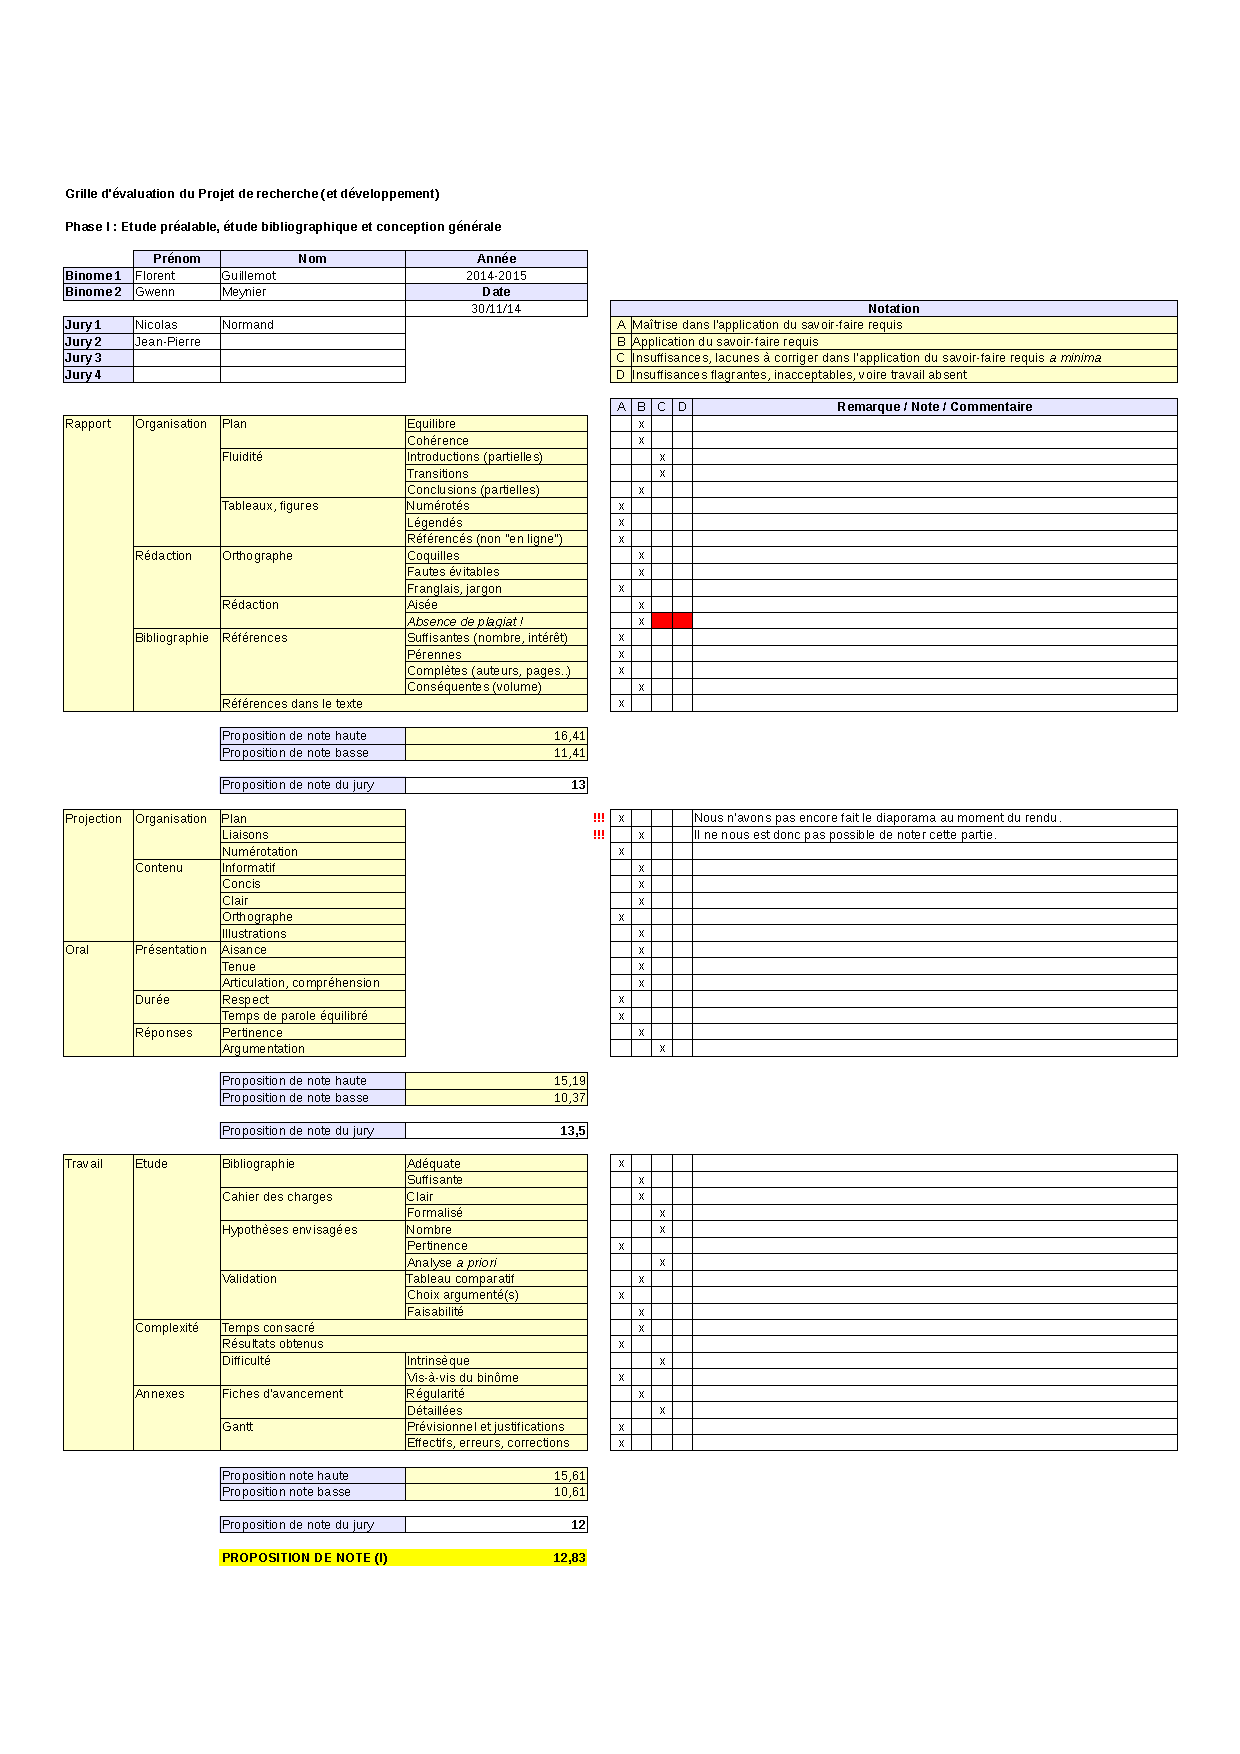
\includegraphics[width=0.9\textheight]{Images/Grille-Evaluation-PRD1}}
      \else
         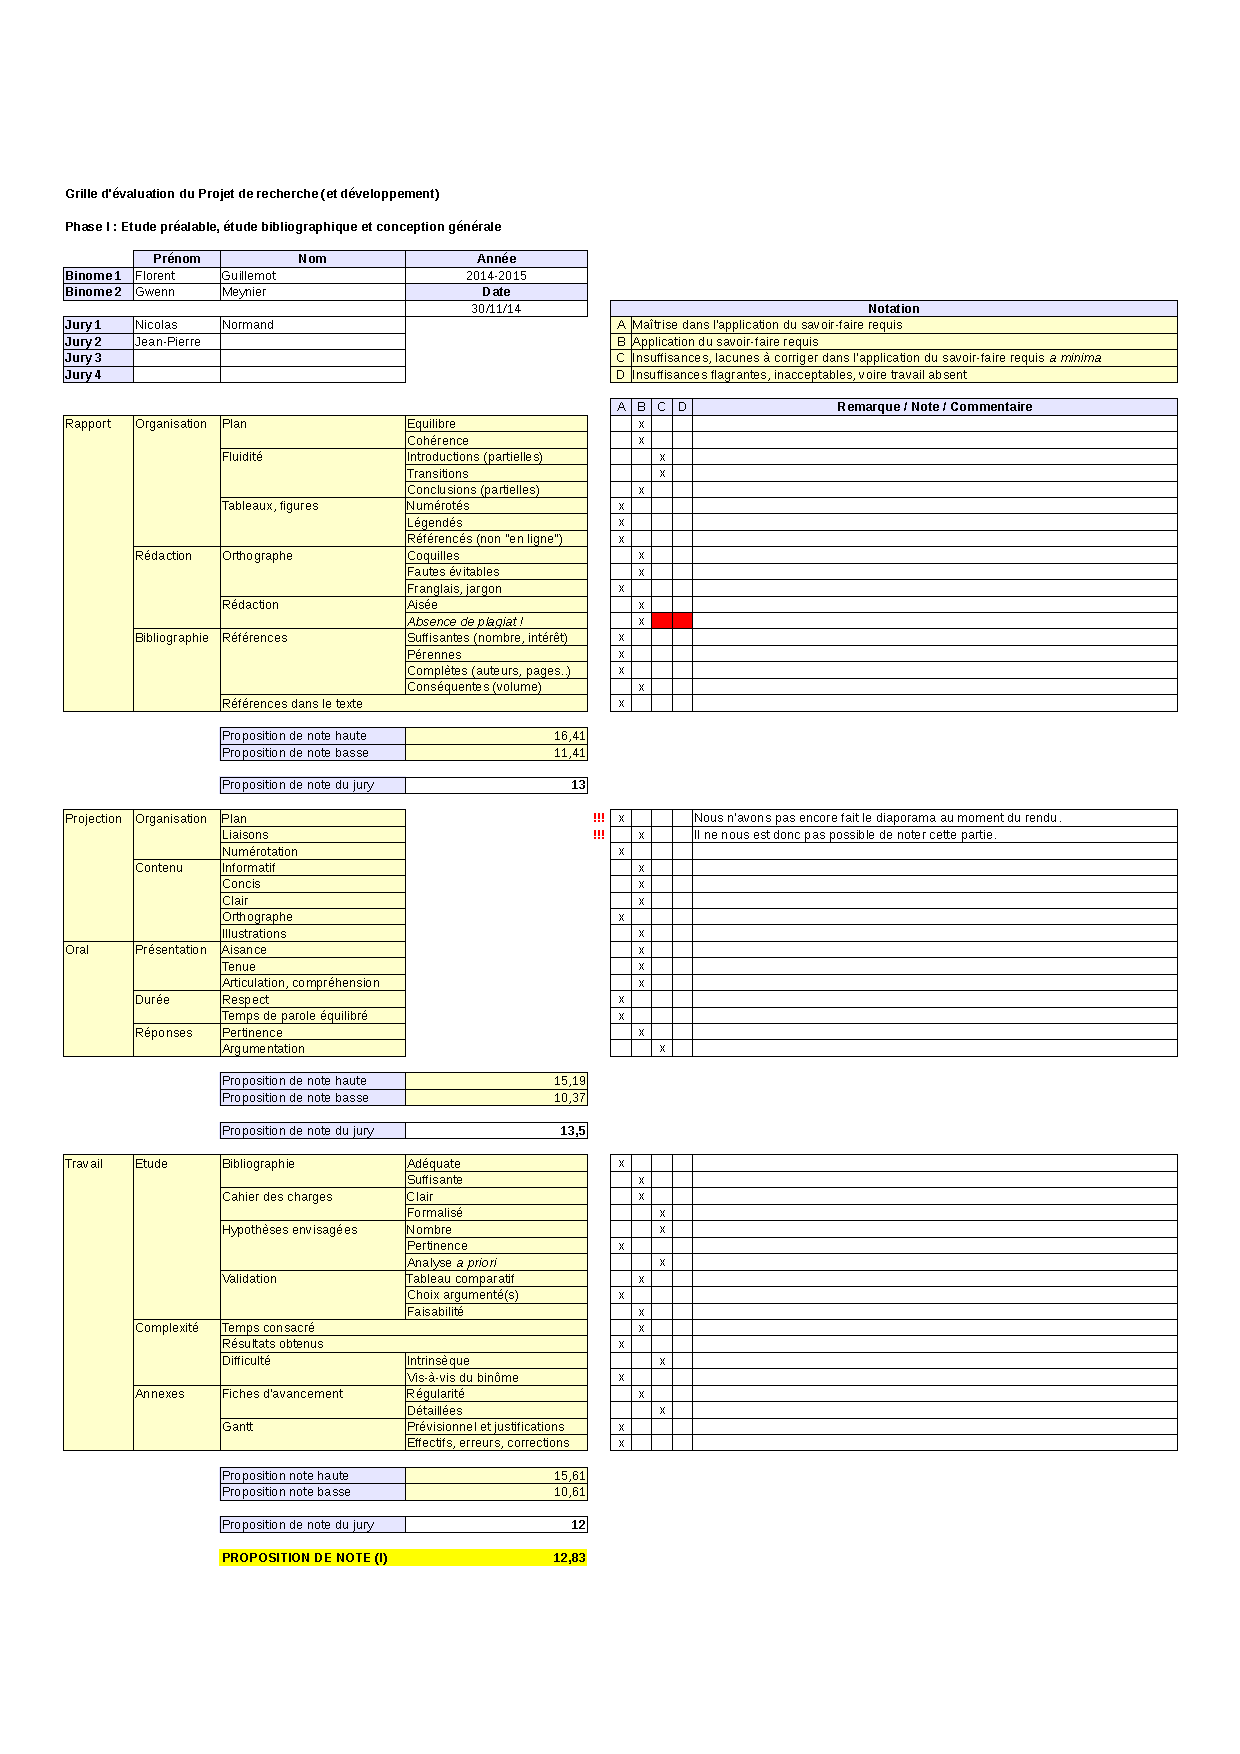
\includegraphics[width=0.9\textwidth]{Images/Grille-Evaluation-PRD1}
      \fi
	\caption{Points à contrôler à l'issue de la phase I}
	\label{fig:AutoEvaluationTravailIntermediaire}
\end{figure*}

La figure~\ref{fig:AutoEvaluationTravailFinal} permet d'énumérer un certain nombre de points importants dans les trois composantes du travail ainsi que d'évaluer notre niveau de satisfaction à l'issue de la phase~II, constituée de :
\begin{enumerate}
	\item la conception détaillée ;
	\item la réalisation ;
	\item la recette.
\end{enumerate}

\begin{figure*}
	\centering
      \ifscreen
         \rotatebox{90}{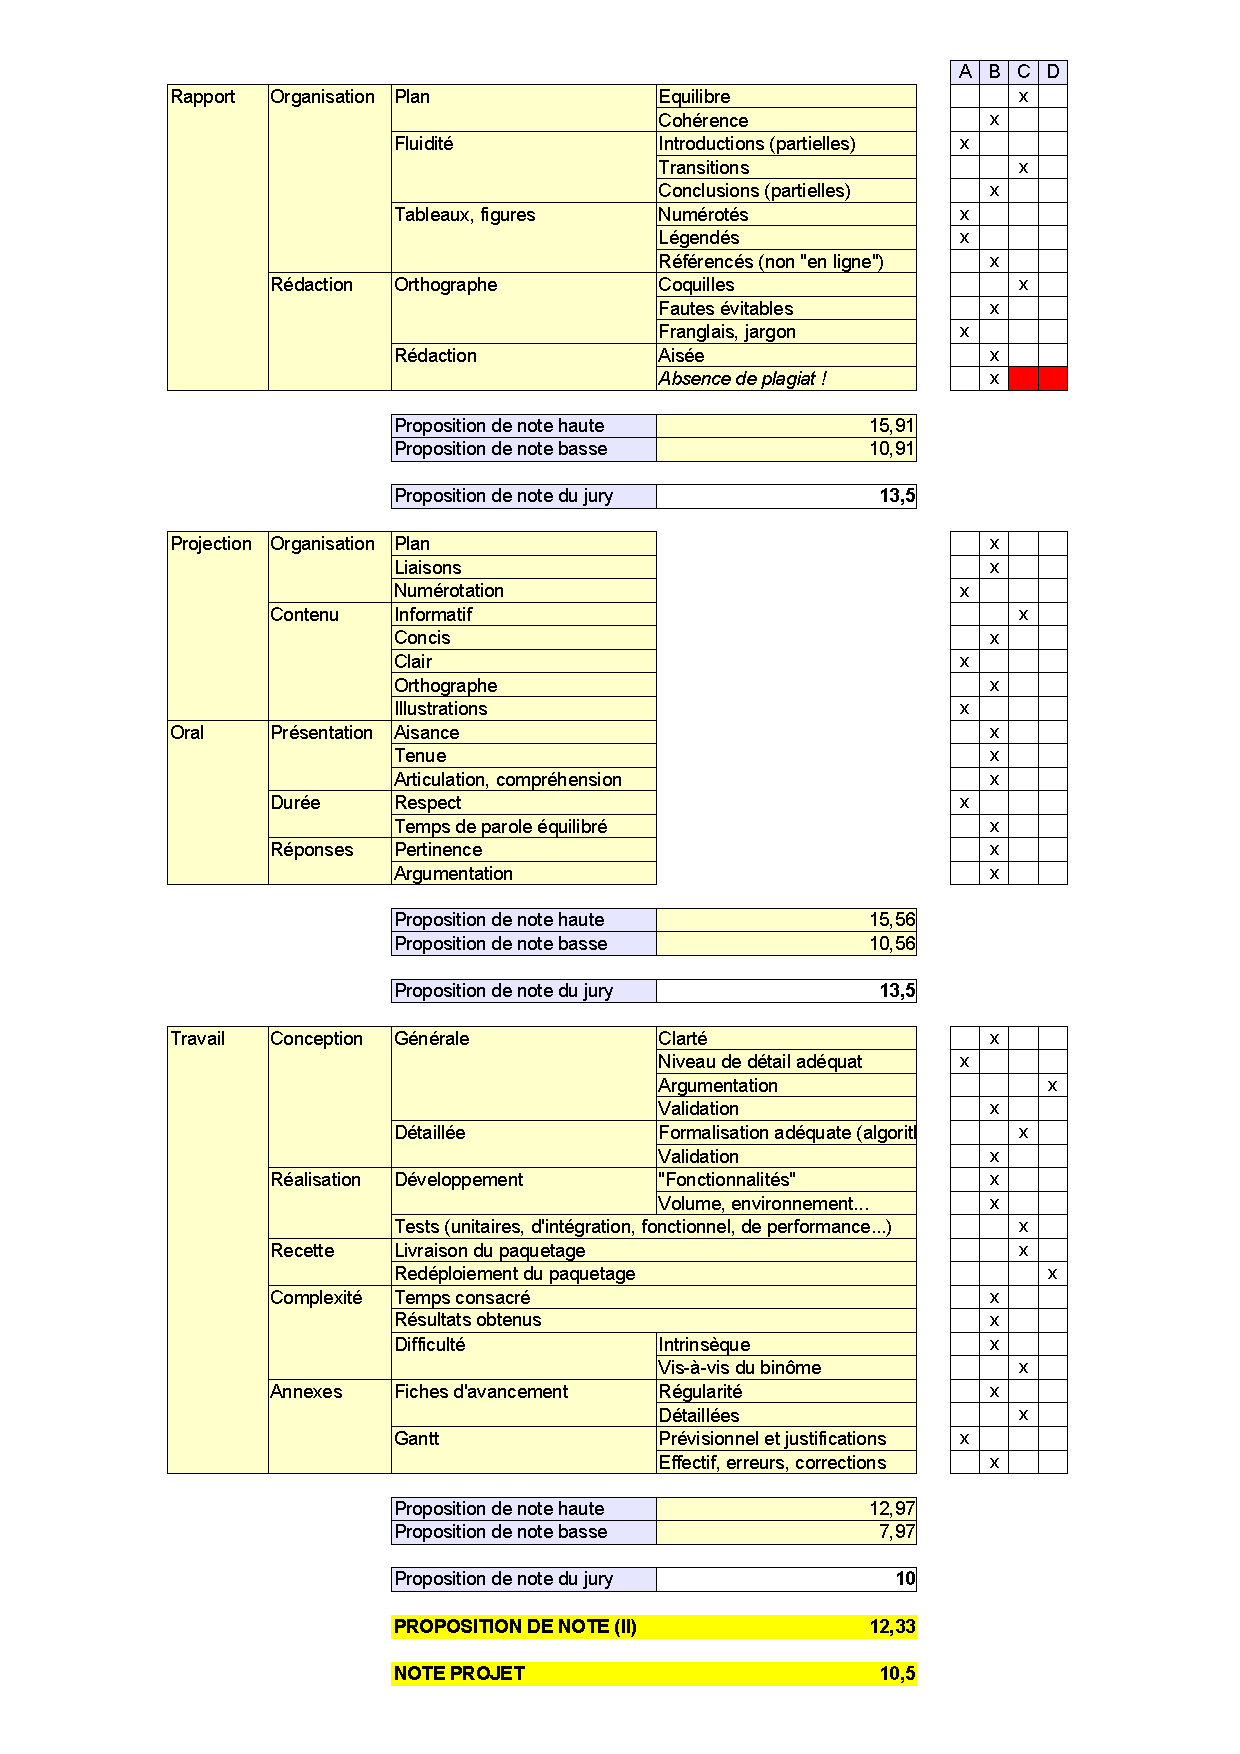
\includegraphics[width=0.9\textheight]{Images/Grille-Evaluation-PRD2}}
      \else
         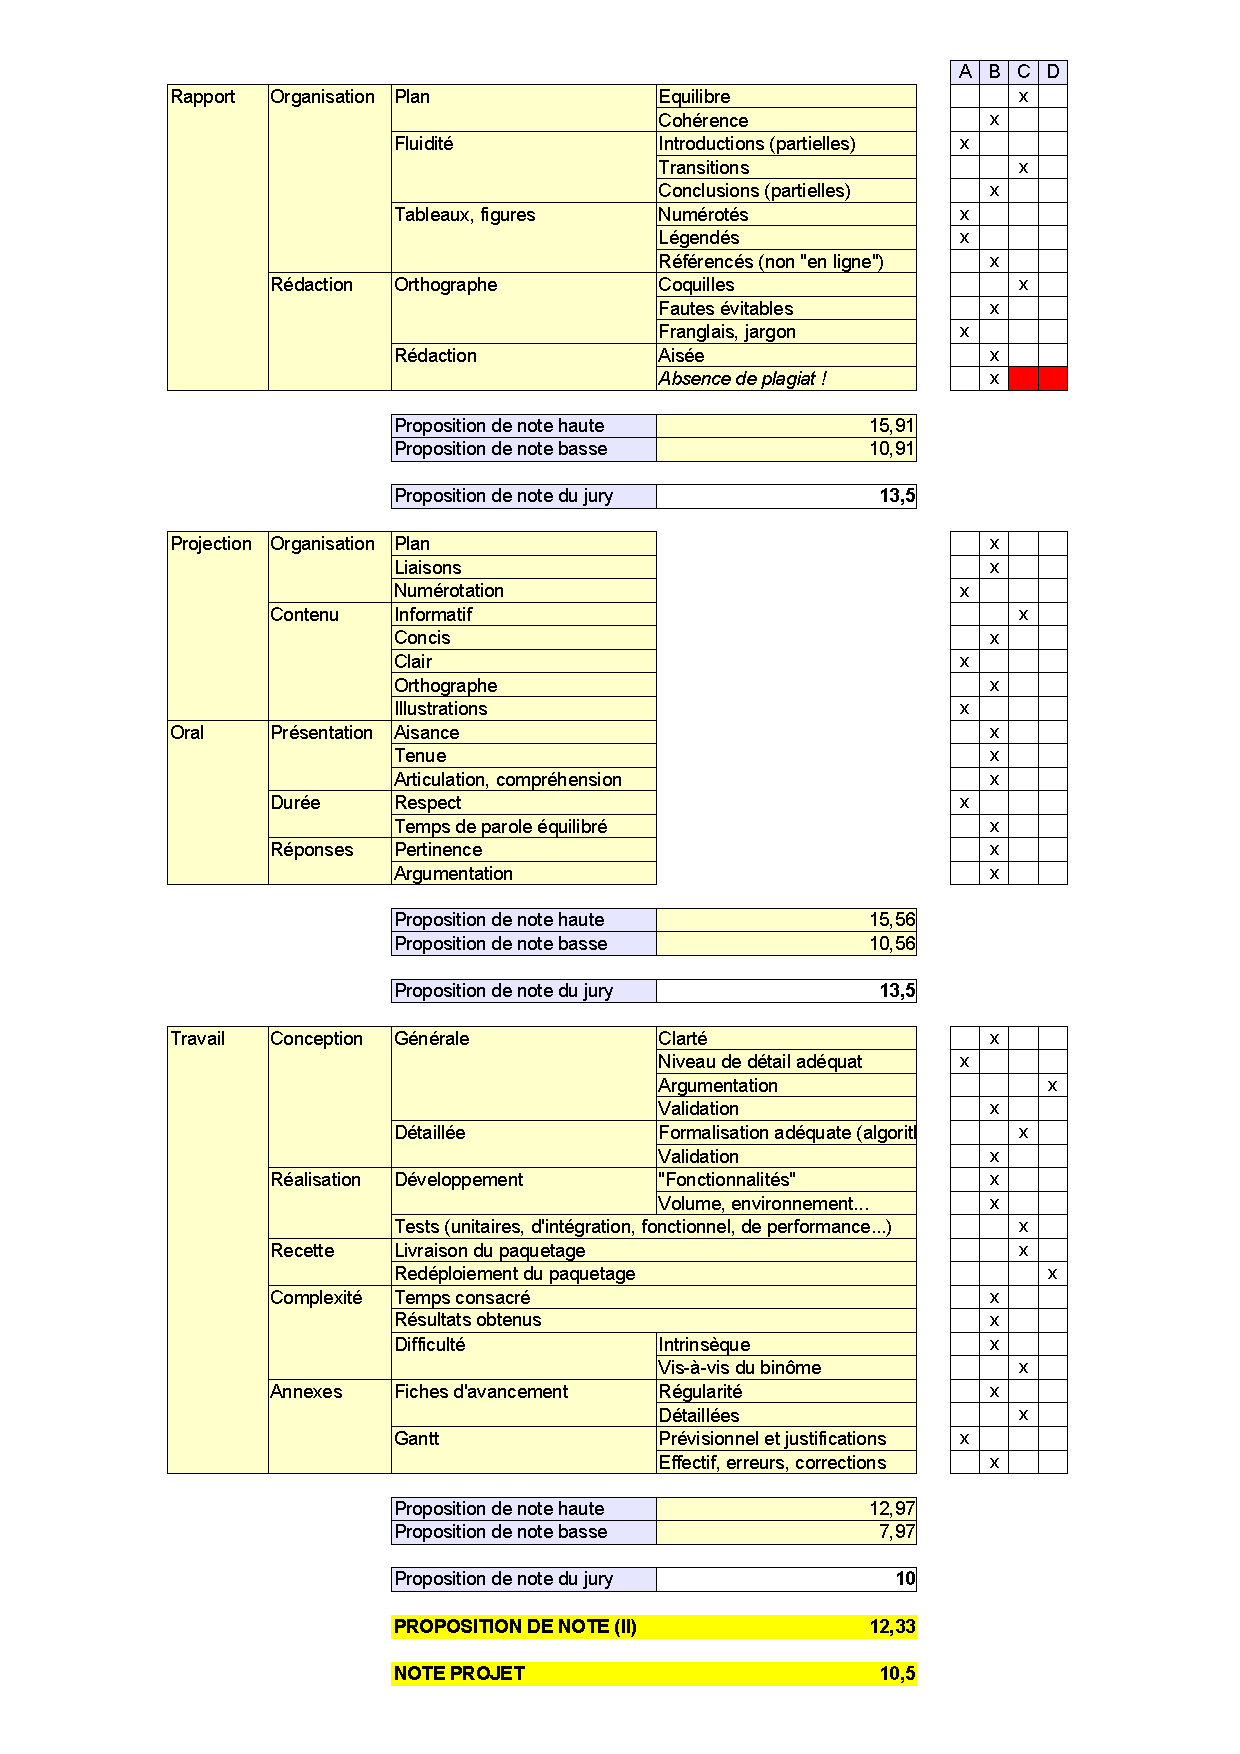
\includegraphics[width=0.9\textwidth]{Images/Grille-Evaluation-PRD2}
      \fi
	\caption{Points à contrôler à l'issue de la phase II}
	\label{fig:AutoEvaluationTravailFinal}
\end{figure*}

\end{document}